\begin{document}

\thispagestyle{empty}

\begin{center}
{\small
МИНОБРНАУКИ РОССИИ\par
ФЕДЕРАЛЬНОЕ ГОСУДАРСТВЕННОЕ БЮДЖЕТНОЕ ОБРАЗОВАТЕЛЬНОЕ\par
УЧРЕЖДЕНИЕ ВЫСШЕГО ОБРАЗОВАНИЯ\par
<<ВОРОНЕЖСКИЙ ГОСУДАРСТВЕННЫЙ УНИВЕРСИТЕТ>>\par
(ФГБОУ ВО <<ВГУ>>)\par
\vspace{4mm}}

Факультет прикладной математики, информатики и механики\par
\vspace{5mm}
Кафедра математического обеспечения ЭВМ\par
\vspace{35mm}

\textbf{Автоматизация разработки и тестирования задач}\par
\textbf{по олимпиадному программированию}\par
\vspace{8mm}

Бакалаврская работа\par
Направление 01.03.02. Прикладная математика и информатика\par
Профиль Системное программирование и компьютерные технологии\par
\end{center}
\vspace{35mm}

Допущен к защите ГЭК \underline{\qquad\qquad\qquad}\par
\vspace{8mm}
Зав. кафедрой \underline{\qquad\qquad\qquad} \qquad\qquad\qquad д.~ф.-м.~н.,~доц.~Махортов~С.~Д.\par
\qquad\qquad\qquad\qquad(подпись)\par
\vspace{2mm}
Обучающийся \underline{\qquad\qquad\qquad} \qquad\qquad\qquad Кузнецов~И.~Э. 4 курс 8 группа\par
\qquad\qquad\qquad\qquad(подпись)\par
\vspace{2mm}
Руководитель \underline{\qquad\qquad\qquad} \qquad\qquad\qquad д.~ф.-м.~н.,~доц.~Махортов~С.~Д.\par
\qquad\qquad\qquad\qquad(подпись)\par
\vspace{11mm}

\begin{center}
Воронеж - 2016
\end{center}

\chapter*{Аннотация}
Олимпиады по программированию сегодня "--- очень распространённое и актуальное явление. Они проводятся как среди школьников, так и среди студентов и профессиональных работников, как на уровне вузов, так и на международном уровне. Многие крупные IT-компании, такие как Google, Facebook, Яндекс, Mail.ru, ВКонтакте, регулярно проводят свои собственные олимпиады.

Проведение олимпиад по программированию требует наличия специального программного обеспечения: тестирующей системы, удовлетворяющей определённому набору требований, а также "--- системы для разработки задач. Подготовка наборов тестов для задач "--- весьма трудоёмкий процесс, требующий применения специальных инструментов, таких как генераторы, валидаторы, чекеры и интеракторы.

В данной работе ставится цель изучить основные аспекты работы тестирующих систем и систем разработки задач для олимпиад по программированию, а также "--- написать программу с удобным графическим пользовательским интерфейсом, предоставляющую возможность разрабатывать новые задачи и проверять решения на подготовленных тестах. Предполагается написание программы на языке Java с использованием библиотеки Swing.

\renewcommand{\contentsname}{Содержание}
\tableofcontents

\chapter*{Введение}
\addcontentsline{toc}{chapter}{Введение}
Олимпиада по программированию "--- это интеллектуальное соревнование по решению различных задач на ЭВМ, для решения которых необходимо придумать и применить какой-либо алгоритм и программу на одном из языков программирования \cite{wiki}. Проводятся такие олимпиады сегодня как среди школьников, так и среди студентов и профессиональных работников, как на уровне вузов, так и на международном уровне. Многие крупные IT-компании, такие как Google, Facebook, Яндекс, Mail.ru, ВКонтакте, регулярно проводят свои собственные олимпиады, что, несомненно, говорит об их актуальности на сегодняшний день.

На олимпиаде по программированию участникам предлагается набор из нескольких задач, решением каждой задачи является программа, написанная на одном из разрешённых языков программирования. Программа должна считывать данные указанного формата из некоторого входного потока, обрабатывать их согласно условию задачи и выводить ответ в выходной поток. Чтобы решение было засчитано как верное, необходимо, чтобы оно выводило правильные ответы на заранее определённом наборе тестов.

Проверка решений на тестах производится с помощью специальных тестирующих систем. Такая система должна уметь компилировать код решений с помощью различных компиляторов, запускать решения на определённых наборах тестов, проверять корректность ответов простым сравнением с эталонными выходными данными или более сложными способами (например, с помощью специальных чекеров), а также "--- выносить вердикты по каждому полученному решению. Кроме того, система должна поддерживать различные системы оценивания решений (такие как IOI~\cite{ioi} и ICPC~\cite{icpc}). Наконец, от тестирующей системы требуется, чтобы она проверяла решения как можно быстрее, для чего, например, проверка может выполняться параллельно в нескольких потоках. Существует несколько известных тестирующих систем, используемых в реальных олимпиадах, например: Ejudge, PCMS2, Contester, Testsys.

Разработка задач для олимпиад по программированию "--- отдельный процесс, который также является весьма трудоёмким. В него входит написание корректного и содержательного условия и подготовка большого набора тестов, которые должны охватывать все возможные частные случаи в задаче. Тесты могут представлять собой данные очень больших объёмов, поэтому для их подготовки также необходимы специальное программное обеспечение и инструменты, такие как генераторы, валидаторы, чекеры и интеракторы, у каждого из которых есть своё особое предназначение. В качестве примера известной системы разработки задач можно привести систему Polygon \cite{polygon}, на которой подготавливают задачи для проведения контестов на платформе Codeforces \cite{codeforces}.

В данной работе мы поставим перед собой цель изучить основные аспекты работы тестирующих систем и систем разработки задач для олимпиад по программированию, а также "--- написать программу с удобным графическим пользовательским интерфейсом, предоставляющую возможность разрабатывать новые задачи и проверять решения на подготовленных тестах. Предполагается написание программы на языке Java с использованием библиотеки Swing.

\chapter{Общетеоретическая часть}
\section{Основные понятия}
На олимпиадном соревновании по программированию участникам предлагается решить несколько задач, каждая из которых представлена набором тестов "--- входных и выходных данных алгоритма, который нужно реализовать. Тесты подготавливаются заранее, и их подготовка "--- довольно длительный процесс. Он подразумевает генерацию входных данных для тестов, их валидацию, а также генерацию выходных данных, написание чекеров и иногда "--- интеракторов \cite{testlib}.

Полное решение задачи "--- работающая программа, которая на каждом тесте даёт правильный ответ. За время соревнования каждому участнику разрешается делать неограниченное количество посылок по каждой задаче различных версий своего решения в тестирующую систему, которая автоматически компилирует решения, запускает их на тестах и выносит для каждой посылки вердикт по определённым правилам. Таким образом, одна посылка участника "--- это файл с исходным кодом программы, вердикт, который тестирующая система присвоила этой посылке, а также "--- общая информация о посылке (максимальное время работы программе на одном тесте, количество использованной памяти и т. д.).

В зависимости от правил проведения того или иного соревнования, участникам могут быть видны вердикты по посылкам, которые они отправляют в тестирующую систему, либо не видны. Часто окончательным решением участника той или иной задачи считается та посылка, которую он отослал позже остальных. Кроме того, участникам может быть доступен общий монитор соревнования, в котором видны текущие результаты по каждой задаче всех остальных участников.

По определённым правилам, в зависимости от используемой на соревновании системы оценивания (IOI~\cite{ioi}, ICPC~\cite{icpc}), каждой задаче присваивается некоторое количество баллов. Они суммируются для каждого участника, и на основе них затем формируется итоговая таблица результатов соревнования.

Таким образом, разработка задач и проверка решений "--- два взаимосвязанных процесса, но рассматривать их можно отдельно друг от друга. Исследуем каждый из них более подробно.
\section{Разработка задач}
Разработка задач "--- это процесс, который происходит задолго до самого соревнования, и его цель "--- подготовить корректные тесты, учитывающие все частные случаи задач. Тестов может быть много, и входные данные каждого из них могут иметь большой размер, поэтому для их генерации пишутся специальные программы "--- генераторы. Для того, чтобы проверить, что входные данные того или иного теста корректны для данной задачи, пишутся валидаторы. Чекеры используются для того, чтобы проверять, является ли ответ участника верным, в тех случаях, когда у задачи может быть много правильных ответов. И, наконец, интеракторы используются в интерактивных задачах, где программа-решение участника может общаться с тестирующей системой, следуя определённому формату ввода-вывода. Последние, впрочем, встречаются нечасто, поэтому мы не будем рассматривать их в нашей работе.

Каждое описанное средство "--- в свою очередь тоже программа. Очевидно, что в каждой из них для многих олимпиадных задач приходится выполнять множество похожих операций. Это подразумевает, что в данном случае целесообразно использование специальной библиотеки, предоставляющей удобные средства для решения типичных задач. Одной из таких библиотек является testlib.h \cite{testlib}, написанная на языке C++. Именно на её характеристики можно опираться при рассмотрении средств разработки задач и в дальнейшем при их написании.

\subsection{Тесты}

Каждый тест представляет собой по крайней мере два файла: входные данные и эталонные выходные данные, предложенные жюри. Почти всегда тесты объединяются в группы, по тем или иным критериям. Это делается, например, для того, чтобы за тесты из разных групп начислять различное количество очков, или чтобы засчитывать тесты из группы только в том случае, когда правильный ответ был получен по всем тестам в группе.

Из всех групп тестов выделяются две, имеющие особое значение: тесты из условия задачи (\texttt{samples}) и претесты (\texttt{pretests}). Тесты из первой группы, в отличие от всех остальных тестов, известны участникам, поскольку содержатся в выданных им условиях задач. Участникам известны как входные данные, так и эталонные выходные данные. Именно используя такие тесты, они могут тестировать свои решения во время соревнования. Как правило, если решение даёт неверный ответ хотя бы на одном тесте из условия, на остальных тестах решение уже не запускается, и за задачу не начисляются очки.

Претесты "--- это тесты, на которых тестируются решения непосредственно во время соревнования. В зависимости от правил проведения соревнования может быть так, что во время соревнования тестирование идёт на всех тестах сразу (например, в ICPC \cite{icpc}), тогда все тесты можно считать претестами. Но в других ситуациях (например, в IOI \cite{ioi} или в контестах на платформе Codeforces \cite{codeforces}) на большей части тестов решения проверяются уже после соревнования, во время так называемого системного тестирования. Это делается для того, чтобы во время соревнования нагружать систему меньшим количеством работы.

Когда сгенерированы входные данные по всем тестам, необходимо также представить эталонные выходные данные жюри. Это делается, как правило, при помощи авторских решений. Автор задачи пишет собственную программу, которая, по его мнению, даёт верные ответы на всех возможных тестах, а затем она запускается для всех входных данных, и полученные выходные данные принимаются как эталонные. Иногда случается так, что во время соревнования в авторском решении находится ошибка, в таких случаях задача считается некорректной, и за неё никому не начисляются очки.

\subsection{Генераторы}

Как уже говорилось ранее, входные данные тестов могут быть очень большими, и далеко не всегда их можно написать вручную. В таких случаях пишутся специальные программы "--- генераторы. Ясно, что при их написании удобно пользоваться уже написанными функциями, выполняющими типичные для генераторов задачи.

Важно, что генераторы, несмотря на простоту их задачи, должны удовлетворять некоторым требованиям. Например, <<генератор должен выводить один и тот же тест при компиляции любым компилятором на любой платформе, если он запущен одинаковым способом>> \cite{testlib}. Это означает, что, во-первых, нельзя использовать стандартные генераторы псевдослучайных чисел, не инициализируя их конкретным значением, потому что так каждый новый вызов генератор будет выдавать разные тесты. И, во-вторых, это значит, что лучше переложить все хлопоты по генерации псевдослучайных значений на используемую библиотеку, чтобы не задумываться об их генерации в момент написания генератора и чтобы библиотека сама обеспечивала однозначность вывода и независимость его от платформы и компилятора.

Таким образом, будет удобно разместить в библиотеке генератор псевдослучайных чисел (для их генерации сойдёт простой линейный конгруэнтный метод), а также "--- предоставить методы для получения, например, целых или дробных чисел из определённого диапазона, символов, удовлетворяющих некоторому шаблону, и т. д.

Кроме того, важно, чтобы генератор был строг к формату выводимого теста, то есть важно, чтобы, например, между числами, символами или словами был только один пробел, чтобы не было лишних пробелов по краям строк, чтобы переводы строки были там, где это ожидается, и чтобы весь тест заканчивался переводом строки. Для того, чтобы это обеспечить, также удобно будет разместить в библиотеке методы для удобного вывода.

Также важно, чтобы генератор мог принимать извне некоторые параметры, например, в виде строковых значений. Это нужно для того, чтобы можно было один и тот же генератор запускать несколько раз с разными входными параметрами и получать различные тесты, удовлетворяющие различным условиям.

\subsection{Валидаторы}

Валидаторы нужны для того, чтобы проверять, что сгенерированные или написанные вручную входные данные для некоторой задачи корректны, то есть удовлетворяют требованиям из условия задачи. Например, может оказаться, что некоторая величина во входных данных превышает допустимое ограничение, или описанный граф не является связным. Подобные вещи может быть сложно оценить с одного взгляда на тест, особенно если входные данные "--- большой файл, созданный генератором. Поэтому, несмотря на то, что валидация тестов, по сути, необязательна, ведь и без неё можно получить корректные тесты и запускать на них решения, проведение валидации настоятельно рекомендуется \cite{testlib}. Более того, написание валидаторов "--- обязательная процедура перед многими контестами, например, перед раундами на платформе Codeforces \cite{codeforces}.

Важно, что валидатор так же, как и генератор, должен быть строг к формату входных данных. Он должен проверять не только то, как расставлены пробелы и переводы строк, но и формат чисел и символов, а в случае какого-либо несовпадения с тем, что ожидалось, выводить удобочитаемое сообщение об ошибке.

Ясно, что в библиотеку разработки задач удобно добавить специальные методы для считывания составных частей входного файла, выполняющие операции вроде следующих: <<прочесть целое число>>, <<прочесть пробел>>, <<прочесть перенос строки>>, <<прочесть конец файла>> и т. д. Полезными могут оказаться также методы проверки, удовлетворяет ли символ или строка некоторому шаблону. Кроме того, удобны методы, позволяющие автоматически сообщать об ошибке, если не выполняется то или иное условие.

Наконец, валидатор так же, как и генератор, должен уметь принимать некоторые параметры, чтобы затем использовать их в своей работе. Это может пригодиться, например, если в разных группах тестов входные данные должны удовлетворять различным ограничениям. Тогда получится использовать один и тот же валидатор с разными параметрами для разных групп тестов.

\subsection{Чекеры}

Как упоминалось ранее, чекеры используются в тех случаях, когда задача имеет множество правильных ответов. Например, в задаче может требоваться вывести описание графа, удовлетворяющего некоторому требованию, или найти кратчайший путь в графе, который также в общем случае может быть не единственным. В таких случаях недостаточно просто сравнить ответ участника с эталонным ответом жюри, поэтому пишутся специальные программы "--- чекеры, которые выполняются непосредственно в момент перед выносом вердикта по посылке и сообщают тестирующей системе о результате проверки.

Чекер должен принимать на входе три потока ввода: для тестовых входных данных, для ответа участника и для ответа жюри. В процессе своего выполнения чекер должен считать и проанализировать данные из каждого потока. При этом чекеру уже не нужно проверять правильность формата тестовых входных данных, потому что эту работу за него уже выполнил ранее валидатор. Следует проверять формат ответа участника, а заодно "--- и ответа жюри.

По итогам своей работы чекер должен вынести вердикт. Чекер может сделать это разными способами. Например, вывести результат в стандартный вывод, в некоторый xml-файл или как-то ещё. В зависимости от реализации и требований к системе можно выделить разные возможные вердикты, мы выделим три основных:

\begin{itemize}
\item \texttt{ACCEPTED} "--- означает, что программой участника был получен правильный ответ, соответствующий необходимому формату вывода.
\item \texttt{WRONG ANSWER} "--- означает, что программа участника либо вывела неправильный ответ.
\item \texttt{PRESENTATION ERROR} "--- означает, что программа участника вывела данные, не соответствующие требуемому формату (данный вердикт часто полностью заменяют предыдущим, потому что во многих случаях сложно определить, какой из них более подходящий).
\item \texttt{FAIL} "--- означает, что при работе чекера произошла непредвиденная ошибка, либо что участником было найден корректный ответ, более оптимальный, чем ответ жюри.
\end{itemize}

Важно, что код чекера также должен удовлетворять определённым требованиям. Во-первых, он не должен предполагать, что ответ жюри абсолютно верен и не подлежит сомнению. То есть если программа участника нашла некоторый формально корректный ответ, который оказался оптимальнее ответа жюри, чекер обязан об этом сообщить. Это должно происходить как раз в том случае, когда в авторском решении была допущена ошибка. Во-вторых, в чекере следует избегать дублирования кода, вынося код считывания ответа в отдельную функцию, чтобы в ней можно было считать как ответ участника, так и ответ жюри. Чекер, написанный таким образом, обычно оказывается короче и проще для понимания и, кроме того, позволяет проверить одновременно формат и ответа участника, и ответа жюри.

Разумеется, в чекере также используется множество операций, которые удобно выполнять, вызывая методы из библиотеки. К таким операциям можно отнести многие операции, которые ранее уже упоминались в разделе о валидаторах, поскольку в чекере часто происходят схожие процессы. Отличие будет состоять в том, что считывание данных из файлов в чекере не должно быть таким строгим, как в валидаторе, поскольку формат выходных данных обычно менее строг. Например, лишние пробелы в выводе не будут критичны, так же, как и перенос строки вместо ожидаемого пробела.
\section{Тестирующие системы}
Задача тестирующей системы "--- обрабатывать полученные посылки, используя подготовленные заранее для каждой задачи тесты. Делать это тестирующая система должна в онлайновом режиме, то есть как только посылка была получена, она сразу должна быть автоматически отправлена на проверку, и как можно быстрее по ней должен быть получен вердикт. Это нужно для того, чтобы непосредственно во время соревнования участники имели возможность видеть результаты той или иной своей посылки и делать из них некоторые выводы.

Таким образом, от тестирующей системы требуется сколь возможно быстрое выполнение её работы, потому что во время соревнование нагрузка на систему может быть очень большой: количество посылок и частота их появления могут быть очень велики. Поэтому при реализации системы используют распараллеливание её задач. Например, можно выделять под проверку каждой новой посылки отдельный поток, потому что проверки двух отдельных посылок никак не зависят друг от друга. В более сложном варианте реализации тестирующей системы отдельный поток выделяется для проверки некоторой посылки на отдельном тесте, но в таком случае необходимо реализовывать приоритизацию потоков выполнения, чтобы одновременно могли проверяться тесты для разных посылок.

Существует определённый алгоритм проверки посылки на тестах, по окончании которого тестирующая система должна присвоить посылке один из возможных вердиктов. Важным понятием является также выбранная система оценивания, от которой зависят многие аспекты работы тестирующей системы, в том числе, например, порядок проверки посылки на отдельных тестах. Кроме того, тестирующая система должна поддерживать использование различных языков программирования и, соответственно, компиляторов, а запуск решений из командной строки в отдельном процессе должен происходить безопасно, чтобы запущенная программа участника не нанесла вред машине, на которой работает сама тестирующая система. Рассмотрим каждый из перечисленных аспектов более подробно.

\subsection{Вердикты}

В общем случае в разных тестирующих системах приняты разные наборы возможных вердиктов, которые система может присвоить полученным посылкам. Перечислим основные виды вердиктов:

\begin{itemize}
\item \texttt{ACCEPTED} "--- означает, что решение дало правильные ответы на всех тестах по задаче и что решение зачтено как верное.
\item \texttt{PRETESTS ACCEPTED} "--- означает, что решение дало правильные ответы на всех претестах. Такой вердикт может быть получен во время соревнования, если после него проводится системное тестирование. Вердикт ещё не значит, что решение зачтено, как верное, потому что во время системного тестирования решение может выдать неправильный ответ на дополнительных тестах. Тогда вердикт будет обновлён.
\item \texttt{PARTIAL ACCEPTED} "--- означает, что решение дало правильные ответы на некоторых тестах и что в итоге всей посылке начислено некоторое количество очков, которое приписывается к данному вердикту дополнительно. Такой вердикт, как правило, может быть получен при системе оценивания IOI, где каждый тест может давать очки независимо от других.
\item \texttt{COMPILATION ERROR} "--- означает, что при попытке скомпилировать исходный код полученного решения произошла ошибка компиляции. В таком случае, разумеется, решение не будет запускаться ни на одном тесте.
\item \texttt{RUNTIME ERROR} "--- означает, что при попытке запустить решение на некотором тесте произошла ошибка времени выполнения, и запущенная программа была завершена с кодом выполнения, отличным от нуля.
\item \texttt{WRONG ANSWER} "--- означает, что на некотором тесте программа-решение полностью отработала, корректно завершилась и выдала некоторый ответ, но тестирующая система расценила данный ответ как неверный (либо он не совпал с эталонным решением, либо используемый в данной задаче чекер дал отрицательный результат).
\item \texttt{PRESENTATION ERROR} "--- означает, что на некотором тесте решение также выполнилось и выдало ответ, но формат ответа не совпал с требуемым в данной задаче. Такой вердикт можно получить в довольно редких случаях. Часто различие между данным вердиктом и вердиктом \texttt{WRONG ANSWER} бывает очень сложно определить, поэтому во многих тестирующих системах от него вообще отказываются и во всех случаях выводят \texttt{WRONG ANSWER}.
\item \texttt{TIME LIMIT} "--- означает, что на некотором тесте решение выполнялось слишком долго и время его выполнения превысило ограничение по данной задаче. В таком случае процесс с выполняемой программой принудительно прерывается и весь её вывод игнорируется.
\item \texttt{MEMORY LIMIT} "--- означает, что на некотором тесте решение потребовало задействовать слишком много памяти, и её количество превысило ограничение по данной задаче. Как правило, в данном случае программа завершается с аварийным кодом выполнения из-за исключения, связанным с нехваткой памяти. Любой вывод программы также игнорируется.
\item \texttt{SECURITY VIOLATED} "--- означает, что на некотором тесте программа-решение попыталась выполнить некоторые действия, запрещённые согласно условиям проведения олимпиады. Например, она могла запросить некоторое свойство операционной системы, обратиться к файловой системе или попытаться создать графический интерфейс.
\item \texttt{FAIL} "--- означает, что в процессе проверки решения произошла некоторая внутренняя ошибка тестирующей системы, из-за которой проверить решение не удалось. Например, аналогичный вердикт мог быть получен в чекере, либо неожиданно пропал тот или иной файл при запуске решения или его компиляции, и т. п.
\end{itemize}

Заметим также, что если вердикт выносится посылке, которая по той или иной причине не прошла все тесты, то к вердикту приписывается также номер первого теста, при проверке которого произошла ошибка. Эта информация также показывается участнику (сам тест, разумеется, остаётся скрытым). Помимо этого почти вместе с каждым вердиктом (где это имеет смысл) записывается ещё максимальное время и максимальная память, потребовавшиеся при обработке одного теста. Эти значения также сообщаются участнику.

Таковы вердикты, которые могут быть вынесены всей посылке в целом. Но помимо этого каждому отдельному тесту при тестировании посылки тоже присваивается некоторый вердикт, а вместе с ним "--- использованные при проверке на одном тесте время и память. Но на некоторых тестах система может вообще не запустить решение (например, если система оценивания "--- ICPC), тогда тесту вообще не присваивается никакого вердикта, либо присваивается специальный вердикт \texttt{NOT TESTED}. Всей посылке в целом обычно присваивается вердикт первого теста, проверка которого не дала положительного результата, либо \texttt{ACCEPTED}, если ни одного такого теста нет.

\subsection{Алгоритм проверки решения}

Как уже говорилось выше, существует вполне определённый алгоритм проверки тестирующей системой одной посылки. Он частично зависит от используемой системы оценивания, но в целом имеет набор чётко выделенных шагов. Вкратце опишем их.

Начинается всё всегда с того, что тестирующая система пытается скомпилировать программу-решение, обращаясь к выбранному компилятору. Если это не удаётся, сразу посылке присваивается вердикт \texttt{COMPILATION ERROR}, и дальше никакие действия по проверке уже не выполняются.

Дальше всегда происходит проверка всех тестов, указанных в условии задачи, то есть тестов из группы \texttt{samples}. Есть правило, что если решение не даёт правильный ответ хотя бы на одном из таких тестов, всегда за решение не начисляются никакие очки. В таком случае сразу присваивается вердикт, аналогичный вердикту за первый неудачный тест.

Далее алгоритм различается в зависимости от системы оценивания. Отличия состоят в порядке запуска решения на тестах, моменте завершения проверки и выносе общего вердикта по посылке. Подробно эти отличия будут описаны ниже, в разделе о системах оценивания.

Проверка решения на одном тесте происходит следующим образом. Вначале засекается текущий момент времени и запускается уже скомпилированная программа, которой передаются во входной поток тестовые входные данные, а в выходной "--- пустой файл. Если время ожидания завершения программы превышает допустимое ограничение, программа прерывается, и тесту присваивается вердикт \texttt{TIME LIMIT}. Если программа завершилась, но с кодом выполнения, отличным от нуля, то вердикт зависит от перехваченного исключения: если ошибка была вызвана нехваткой памяти, будет вердикт \texttt{MEMORY LIMIT}, или нарушением безопасности, "--- вердикт \texttt{SECURITY VIOLATED}, а в любом другом случае "--- \texttt{RUNTIME ERROR}.

Если программа выполнилась успешно (с кодом выполнения, равным нулю) и от неё были получены выходные данные, то запускается проверка этих данных. Либо происходит сравнение вывода с эталонным ответом жюри, либо запускается чекер. В обоих случаях возможно получение одного из четырёх вердиктов: \texttt{ACCEPTED}, \texttt{PRESENTATION ERROR}, \texttt{WRONG ANSWER} и \texttt{FAIL} "--- согласно описанию результатов работы чекера в одном из предыдущих разделов. Соответствующий вердикт присваивается данному тесту.

Кроме того, вердикт \texttt{FAIL}, как уже говорилось выше, также может быть присвоен посылке в любой ситуации, когда тестирующая система не смогла корректно завершить проверку посылки.

\subsection{Системы оценивания}

Существует две самые известные системы оценивания: IOI~\cite{ioi} и ICPC~\cite{icpc}. Первая широко используется на олимпиадах школьников, а вторая "--- на студенческих олимпиадах. От используемой системы оценивания зависит то, каким образом будут ранжироваться участники в таблице результатов соревнования. Кроме того, она также влияет на вынос вердиктов по посылкам и на порядок запуска решения на тестах. Существуют также и другие системы оценивания, например, на платформе Codeforces \cite{codeforces} используется своя система оценивания, во многом похожая на ICPC, но в данной работе мы не будем её рассматривать.

Если используется система оценивания ICPC, решение засчитывается верным только в том случае, если оно даёт правильные ответы на всех тестах. По итогам соревнования для каждого участника известно, какие задачи он решил, а также "--- в какой момент времени и с какой попытки он решил каждую задачу. За каждую задачу участнику начисляется штрафное время, которое вычисляется как количество минут от начала соревнования до отправки посылки с верным решением, плюс количество неудачных посылок, умноженное на двадцать минут. Штрафы суммируются по всем задачам для каждого участника, и затем все участники ранжируются в первую очередь по количеству решённых задач в порядке невозрастания, а затем "--- по штрафному времени в порядке неубывания. Таким образом получается итоговая таблица.

Как правило, соревнования такого формата проводятся без системного тестирования, то есть задачи проверяются на всех тестах непосредственно во время соревнования, и участники могут сразу видеть итоговый вердикт по своим посылкам, который в дальнейшем уже не изменится. Заметим, что так как вердикт \texttt{ACCEPTED} может быть присвоен посылке только при успешном прохождении всех тестов, если решение не прошло хотя бы один тест, все последующие проверять уже нет смысла, и тогда тестирующая система сразу выносит вердикт, аналогичный вердикту за первый неудачный тест.

Другая схема используется в системе оценивания IOI. Некоторые условия проведения олимпиад школьников могут различаться от случая к случаю, но общие правила таковы. За каждую задачу можно получить максимум некоторое количество баллов, обычно это количество равно 100. Баллы начисляются в зависимости от того, какие тесты и из какой группы успешно прошли тестирование. Для некоторых групп можно указать правило, что баллы за тесты из группы начисляются только в том случае, когда были успешно пройдены все тесты из группы, а для других "--- правило, что тесты оцениваются независимо друг от друга. Окончательным решением задачи считается последняя отправленная участником посылка по данной задаче. Таким образом, каждый участник получает за каждую задачу некоторое количество баллов. В итоговой таблице участники ранжируются в порядке невозрастания только по одному значению "--- суммарному количеству набранных баллов по всем задачам.

По той причине, что тесты могут оцениваться независимо друг от друга, в отличие от ситуации при ICPC, здесь приходится проверять решение на всех тестах вне зависимости от вердиктов, присвоенных им. Как правило, удобно выводить один и тот же вердикт для всех посылок, которые прошли обязательные тесты из группы \texttt{samples}: вердикт \texttt{PARTIAL ACCEPTED} с приписанным ему количеством набранных баллов.

\subsection{Запуск решения}

Последний момент, о котором необходимо упомянуть, "--- это то, каким образом правильно запускать решения участников. Это во многом зависит от используемых участником языка программирования и компилятора, поскольку в использовании каждого компилятора есть свои особенности и нюансы.

В описании каждой задачи должно значиться два значения: количество миллисекунд и количество мегабайт, которые тестирующая система даёт в распоряжение программе-решению на её выполнение. Таким образом, нужно уметь отслеживать время, которое программа потратила на своё выполнение, и прерывать её, если она превысила заданное ограничение. А также нужно уметь ограничить программу в плане потребления памяти.

Помимо этого необходимо передать программе входные и выходные данные. Это можно делать двумя разными способами: либо программе перенаправляют файлы для ввода и вывода в стандартные входной и выходной поток (тогда участники могут работать с ними, как с консолью), либо участникам сообщаются имена входного и выходного файлов, и они из кода своей программы самостоятельно обращаются к их содержимому. Стоит заметить, что первый способ часто оказывается удобнее, как в плане реализации тестирующей системы (не нужно отслеживать, к каким файлам программа-решение должна иметь доступ), так и в плане написания решения участниками, так как им не приходится тратить время на написание кода для доступа к файлам.

Наконец, необходимо ещё отследить, чтобы программа участника не выполнила никаких противоправных действий и не нанесла ущерба тестирующей системе. Как правило, запускаемой программе дают минимум возможных прав, так как для решения олимпиадной задачи никакие особенные права не нужны. Обычно участникам запрещено в коде своих решений выполнять следующие действия:

\begin{itemize}
\item получать доступ к сети;
\item работать с директориями и файлами кроме тех, что определены в условии задачи;
\item считывать и изменять системные свойства;
\item запускать другие программы и создавать новые процессы;
\item создавать какие-либо компоненты графического интерфейса и манипулировать ими;
\item работать с внешними устройствами ввода-вывода;
\item работать с реестром операционной системы.
\end{itemize}

\chapter{Практическая часть}
\section{Постановка задачи}
Цель данной работы "--- написать программу с графическим пользовательским интерфейсом, предоставляющую определённые средства для разработки задач по олимпиадному программированию и для тестирования решений к созданным задачам. Рассмотрим основные варианты использования, которые необходимо реализовать. Так как разработку задач и тестирование решений можно рассматривать отдельно, варианты использования изображены ниже на двух отдельных диаграммах.

На рис.~\ref{use_case_diagram_development} изображена диаграмма вариантов использования, связанных с разработкой задач. Предполагается возможность прикреплять к задаче определённые параметры (такие, как ограничения по времени и памяти, условие задачи), а также "--- тесты, генераторы, валидаторы, чекеры и авторские решения (подробнее обо всём этом речь пойдёт в следующей главе).

\begin{figure}[h]
\center{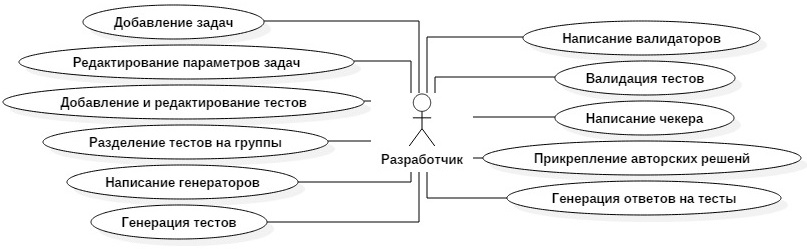
\includegraphics[scale=0.8]{use_case_diagram_development}}
\caption{Варианты использования (разработка задач)}
\label{use_case_diagram_development}
\end{figure}

Создаваемое приложение должно давать возможность писать код для генераторов, валидаторов и чекеров прямо в своём графическом интерфейсе. Это предполагает также написание специальной библиотеки для разработки задач. Эта библиотека будет предоставлять методы с реализацией типичных операций, и пользователь сможет вызывать их прямо из своего кода. Кроме того, все перечисленные средства разработки можно будет компилировать и запускать из самого приложения.

Диаграмма на рис.~\ref{use_case_diagram_testing} отражает варианты использования, связанные с тестированием решений. Заметим здесь, что предполагается возможность отправлять решения, написанные на разных языках: в данной работе мы реализуем поддержу всего двух языков программирования "--- Java и C++. Также приложение должно будет поддерживать различные системы оценивания (их мы также подробно рассмотрим в следующей главе).

\begin{figure}[h]
\center{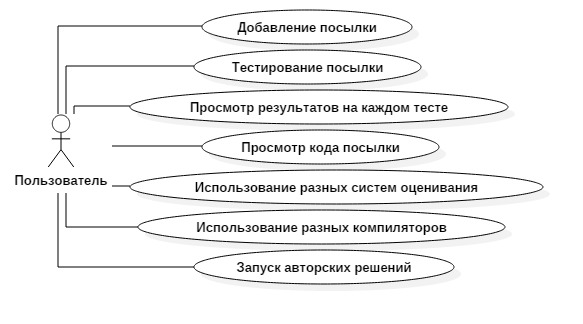
\includegraphics[scale=0.65]{use_case_diagram_testing}}
\caption{Варианты использования (тестирование)}
\label{use_case_diagram_testing}
\end{figure}

Приложение будет сохранять всю информацию в файловой системе и не будет использовать никаких баз данных. По определённому пути, который пользователь сможет выбрать, будет находиться определённая иерархия папок, в которых будут храниться все создаваемые и отправляемые файлы: условия задач, тесты, генераторы, валидаторы, чекеры, авторские и прочие решения, конфигурационные файлы. Все параметры, которые будут прикрепляться к задачам и решениям, будут также храниться в файловой системе в XML-дескрипторах.
\section{Средства реализации}
В качестве языка программирования для реализации приложения выбран язык Java. Такой выбор объясняется удобством использования объектно-ориентирован-ного программирования в данном языке и, следовательно, "--- удобством реализации паттернов проектирования~\cite{gamma}, которые будет уместно применить для расширяемости приложения.

При разработке приложения были использованы различные полезные технологии. Ниже приведён полный список использованных технологий:

\begin{itemize}
\item JDK 1.8~\cite{java} "--- выбрана версия 1.8, поскольку в ней поддерживаются лямбда-выражения, которые было весьма удобно использовать при реализации;
\item Swing "--- использован для реализации графического интерфейса;
\item JUnit 4 "--- использован для написания нескольких юнит-тестов приложения;
\item Git "--- использован в качестве системы контроля версий;
\item GitHub "--- использован для хранения репозитория;
\item Maven "--- использован в качестве фреймворка для сборки проекта;
\item NetBeans 8.1 "--- данная IDE предоставляет как гибкие средства для редактирования и рефакторинга кода, так и удобный инструментарий для создания графического интерфейса при помощи библиотеки Swing.
\end{itemize}
\section{Библиотека для разработки задач}
Библиотека для разработки задач.

\begin{figure}[h]
\center{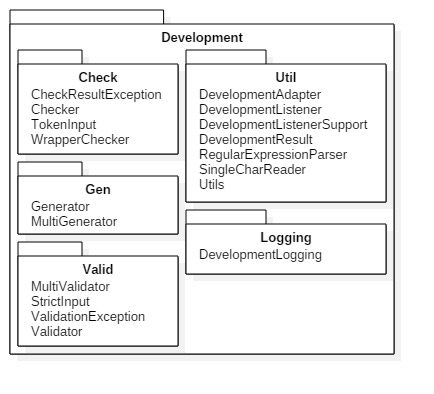
\includegraphics[scale=0.8]{package_diagram_development}}
\caption{Модуль для разработки задач}
\label{package_diagram_development}
\end{figure}
\section{Тестирующий модуль}
Классы модуля тестирования также разделены на пакеты. Отдельный пакет отведён под классы, отвечающие за использование разных языков программирования, систем оценивания, способов проверки корректности ответа, за алгоритм тестирования, за распараллеливание процесса тестирования, а также за регистрирование объектов, доступных для использования в системе, и за логирование. Схема распределения классов в модуле тестирования отображена на рис.~\ref{package_diagram_testing}.

\begin{figure}[h]
\center{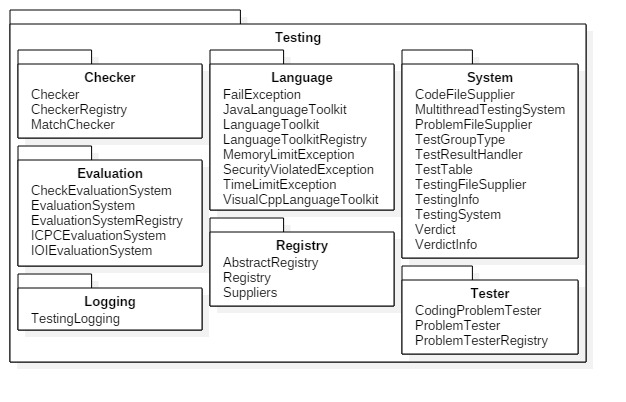
\includegraphics[scale=0.8]{package_diagram_testing}}
\caption{Модуль тестирования}
\label{package_diagram_testing}
\end{figure}

Центральное место в модуле занимают интерфейс \texttt{Testing\-System} и его реализация \texttt{Multithread\-Testing\-System}, которые принимают объекты класса \texttt{Tes\-ting\-Info} со всей необходимой информацией о посылке и ставят их в очередь на проверку (см. рис.~\ref{class_diagram_multithread}). В классе \texttt{Multithread\-Testing\-System} происходит распараллеливание процесса проверки, благодаря чему каждая посылка проверяется в отдельном потоке. Вся работа по управлению потоками ложится на класс \texttt{Executor\-Completion\-Service} из стандартной библиотеки~\cite{cornell1}. При этом на этапе инициализации возможно установить максимальное количество потоков, которым будет разрешено работать одновременно, так, чтобы появляющиеся новые посылки оставались в очереди и ожидали момента, когда для них освободится место. При инициализации объект этого класса также получает реализацию интерфейса \texttt{Testing\-File\-Supplier}, предоставляющего методы для работы с временными и конфигурационными файлами.

\begin{figure}[h]
\center{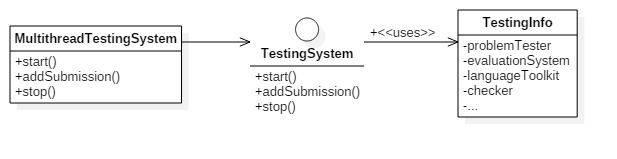
\includegraphics[scale=0.75]{class_diagram_multithread}}
\caption{Интерфейс \texttt{TestingSystem} с реализацией}
\label{class_diagram_multithread}
\end{figure}

Также в системе запущен отдельный поток, в котором поочерёдно для каждой посылки после её проверки будут обрабатываться результаты посредством вызова заданной callback-функции (реализации интерфейса \texttt{Test\-Result\-Handler}). Поскольку этот процесс происходит в одном потоке, исключаются конфликты из-за конкурентного доступа в других модулях.

По окончании тестирования посылки ей присуждается некоторый вердикт с дополнительный информацией, которые записываются в объект класса \texttt{Verdict\-Info}. В нём хранится объект перечислимого типа \texttt{Verdict} (в нём перечислены все возможные вердикты, упомянутые в одной из предыдущих глав), а также максимальные время и память, затраченные решением за одном тесте, количество присуждённых очков и номер первого теста, который решение не прошло успешно, если это произошло. Такой же объект \texttt{Verdict\-Info} ставится в соответствие каждому тесту и записывается в объект класса \texttt{Test\-Table}, в котором хранится заранее подготовленная таблица с информацией о том, сколько тестов находится в каждой группе тестов.

Объект класса \texttt{Testing\-Info}, добавляемый в систему на проверку, должен быть подготовлен заранее один раз, и после отправки вызывающий код может больше не заботиться о нём. Важно только записать в него всю необходимую информацию для обработки посылки. Помимо некоторой общей информации о посылке (ограничения по времени и по памяти, которые нужно применить при тестировании, необходимости проверки только на претестах и подготовленного объекта класса \texttt{Test\-Table}) нужно также предоставить реализации следующих интерфейсов:

\begin{itemize}
\item \texttt{ProblemTester} "--- применяемый алгоритм проверки;
\item \texttt{EvaluationSystem} "--- применяемая система оценивания;
\item \texttt{LanguageToolkit} "--- выбранный язык программирования;
\item \texttt{Checker} "--- применяемый в задаче способ проверки правильности ответа;
\item \texttt{CodeFileSupplier} "--- предоставляет методы доступа к путям, по которым нужно искать файл с исходным кодом и располагать скомпилированный файл;
\item \texttt{ProblemFileSupplier} "--- предоставляет методы доступа к путям, по которым расположены тесты к задаче и скомпилированный файл чекера;
\item \texttt{TestResultHandler} "--- callback-функция для обработки результата тестирования посылки.
\end{itemize}

Рассмотрим первые четыре интерфейса более подробно. Начнём с интерфейса \texttt{Problem\-Tester}. В модуле предоставлена единственная его реализация "--- класс \texttt{Coding\-Problem\-Tester}, реализующий типичный алгоритм тестирования посылки на олимпиаде по программированию. Этот алгоритм, совмещённый с логикой системы оценивания ICPC, в общих чертах изображён на activity-диаграмме на рис.~\ref{activity_diagram_testing}. Он вполне согласуется с тем алгоритмов, что был описан в одной из предыдущих глав.

Класс \texttt{Coding\-Problem\-Tester} общается с системой оценивания (реализацией интерфейса \texttt{Evaluation\-System}) посредством передачи ей объекта класса \texttt{Coding\-Tester\-Delegate} (см. рис.~\ref{class_diagram_testing}) с методами для запуска тестирования посылки на определённом тесте, чтобы обеспечить системе оценивания возможность определить порядок проверки. Таким образом, поддерживается различный порядок запуска решения на тестах при разных системах оценивания.

\begin{figure}[!p]
\center{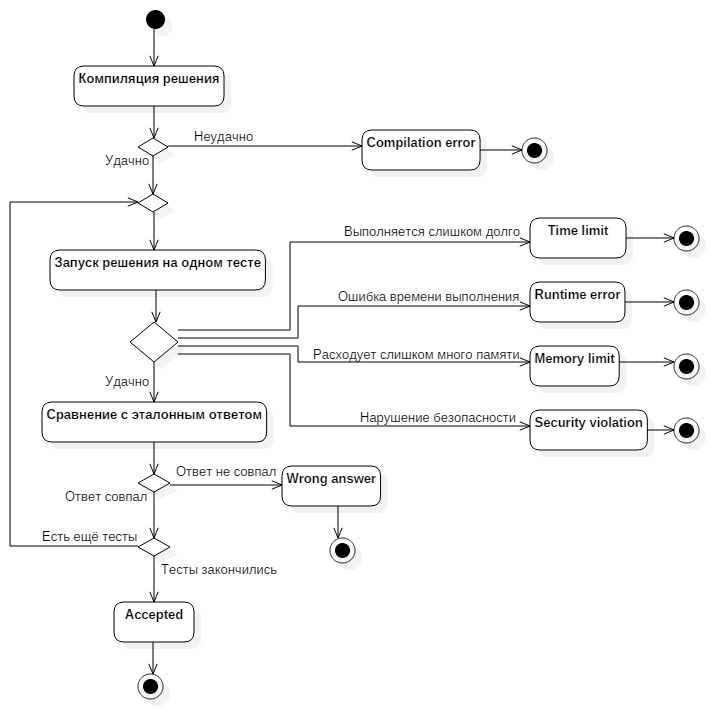
\includegraphics[scale=0.75]{activity_diagram_testing}}
\caption{Алгоритм тестирования посылки}
\label{activity_diagram_testing}
\end{figure}

\begin{figure}[!p]
\center{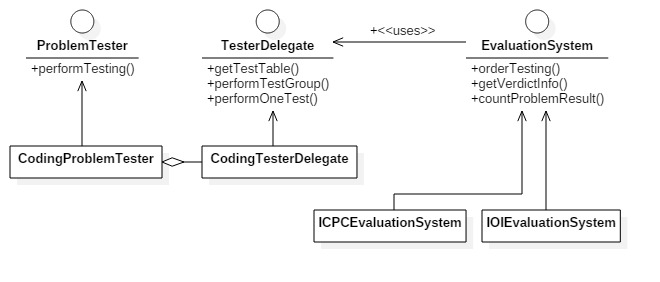
\includegraphics[scale=0.65]{class_diagram_testing}}
\caption{Взаимодействие интерфейсов \texttt{ProblemTester} и \texttt{EvaluationSystem}}
\label{class_diagram_testing}
\end{figure}

Интерфейс \texttt{Evaluation\-System} имеет всего три метода: для определения порядка тестирования, для определения вердикта по посылке и для вычисления количества очков и штрафа по задаче на основе информации обо всех посылках, сделанных по данной задаче. В данном модуле присутствует три реализации этого интерфейса: \texttt{ICPC\-Evaluation\-System}, \texttt{IOI\-Evaluation\-System} (соответствующие двум реальным системам оценивания) и \texttt{Check\-Evaluation\-System} (специальная реализация для принудительной проверки посылки на всех тестах).

Интерфейс \texttt{Language\-Toolkit} (см. рис.~\ref{class_diagram_languages}) содержит два метода: для компиляции исходного кода и для выполнения программы. Заметим, что именно на уровне реализаций данного интерфейса происходит отлавливание всех исключительных ситуаций, изображённых на рис.~\ref{activity_diagram_testing}. Благодаря запуску решения в отдельном процессе появляется возможность прервать его выполнение в любой момент. Присутствует две реализации "--- соответственно для языков Java и C++.

\begin{figure}[h]
\center{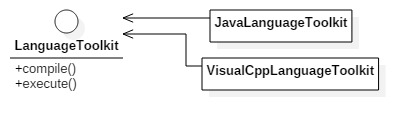
\includegraphics[scale=0.9]{class_diagram_languages}}
\caption{Интерфейс \texttt{LanguageToolkit} с реализациями}
\label{class_diagram_languages}
\end{figure}

Класс \texttt{Java\-Language\-Toolkit} берёт из конфигурационного файла \texttt{java.pro\-perties} путь к установленному на компьютере JDK, а из файла \texttt{java\_problem.po\-licy} "--- список прав (пустой), присуждаемых запускаемым программам-решениям на языке Java. Компиляция Java-кода происходит с помощью специального API, имеющегося в JDK.

Класс \texttt{Visual\-Cpp\-Language\-Toolkit} для компиляции кода на C++ использует компилятор, поставляемый вместе со средой разработки Microsoft Visual Studio. Для этого используется конфигурационный файл \texttt{visual\_cpp.properties}. В нём прописывается путь к папке с компилятором и bat-файлом, который необходимо выполнить перед запуском компилятора. Как для компиляции, так и для выполнения скомпилированной программы запускается отдельный процесс.

Интерфейс \texttt{Checker} соответствует способу проверки правильности ответа участника на основе содержимого трёх файлов: входных данных, ответа участника и ответа жюри. По сути, он соответствует одноимённому классу из библиотеки для разработки задач, но напрямую с ним не связан (их связь реализована в модуле взаимодействия с пользователем). Зато в данном модуле есть реализация этого интерфейса по умолчанию "--- класс \texttt{MatchChecker}, "--- которая может использоваться в случаях, когда ответ в задаче единственен. Эта реализация просто проверяет на равенство ответ участника и эталонный ответ жюри.

Наконец, в данном модуле присутствует система реестров, реализующих интерфейс \texttt{Registry} и расширяющих абстрактный класс \texttt{AbstractRegistry}. Они нужны для того, чтобы хранить в них способы получения реализаций некоторых интерфейсов из данного модуля, поставленные в соответствие строковым идентификаторам. Таким образом, вызывающий код получает удобное решение в случае необходимости получить ту или иную реализацию.
\section{Модуль для работы с файловой системой}
Модуль для работы с файловой системой.
\section{Модуль с графическим интерфейсом}
Модуль с графическим интерфейсом.
\section{Пример работы приложения}
Рассмотрим работу нашего приложения на примере подготовки такой простой задачи: необходимо для некоторого целого числа $n$ ($2 \leq n \leq 10^{12}$) определить, является ли оно простым, и если является, вывести -1, а в противном случае "--- произвольный его делитель, отличный от единицы и самого числа $n$. Заметим, что в задаче правильный ответ может быть не единственным, поэтому необходимо писать код для чекера. Также мы рассмотрим процесс генерации и валидации тестов, прикрепления авторского решения к задаче и отправки посылки.

На рис.~\ref{screen_problems} отображена вкладка главного окна программы со списком всех созданных задач. Здесь можно добавить или удалить задачу, а также перейти к её редактированию. Как можно видеть, задача <<Prime checking>> уже добавлена.

\begin{figure}[h]
\center{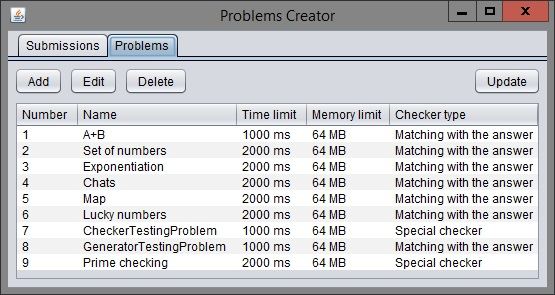
\includegraphics[scale=0.9]{screen_problems}}
\caption{Список созданных задач}
\label{screen_problems}
\end{figure}

Если выбрать задачу и нажать на кнопку <<Edit>>, откроется новое окно с шестью вкладками для редактирования выбранной задачи. На рис.~\ref{screen_problem_param} показана вкладка с основными параметрами задачи: названием, ограничениями по времени и памяти. Также здесь можно загрузить новый файл с условием. Мы выберем ограничения, равные двум секундам и 64-м мегабайтам.

На следующей вкладке (рис.~\ref{screen_tests}) можно посмотреть списки тестов, распределённые по группам, которые можно выбирать в выпадающем списке. Здесь можно добавить или удалить тест, просмотреть входные и выходные данные теста, чтобы изменить их вручную, а также "--- указать количество очков, присуждаемое за один тест из данной группы.

\begin{figure}[h]
\center{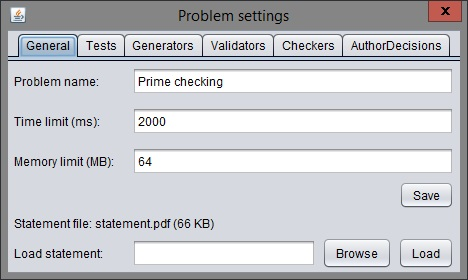
\includegraphics[scale=0.9]{screen_problem_param}}
\caption{Основные параметры задачи}
\label{screen_problem_param}
\end{figure}

\begin{figure}[h]
\center{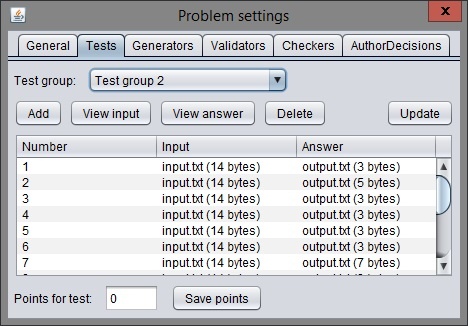
\includegraphics[scale=0.9]{screen_tests}}
\caption{Группа тестов в задаче}
\label{screen_tests}
\end{figure}

\begin{figure}[!ht]
\center{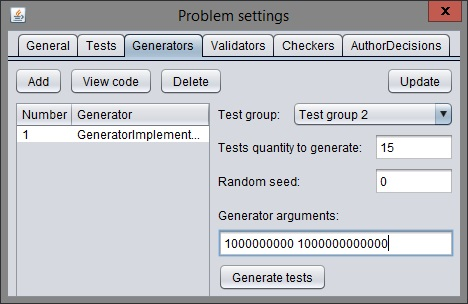
\includegraphics[scale=1.0]{screen_generators}}
\caption{Указание параметров запуска генератора}
\label{screen_generators}
\end{figure}

На вкладке <<Generators>> (рис.~\ref{screen_generators}) можно просмотреть список созданных для этой задачи генераторов, добавить новый (при этом копируется пустой шаблон для генератора) или удалить старый, а также изменить код. На этой же странице можно запускать генератор. Для этого нужно выбрать группу тестов, в которую затем нужно будет сохранить сгенерированные файлы, количество создаваемых тестов, инициализирующее значение для генератора псевдослучайных чисел и строковые параметры генератора, разделённые пробелом.

При нажатии на кнопку <<View code>> открывается окно, отображённое на рис.~\ref{screen_generator_code}. Такое же окно открывается для просмотра и изменения содержимого всех остальных файлов. В данном случае в нём доступен режим редактирования. Для данной задачи достаточно простейшего генератора, принимающего два числовых параметра для определения границ диапазона, в котором должно находиться число $n$ из входных данных, и генерирующего это число.

На рис.~\ref{screen_generator_result} показано окно, которое появится, если мы запустим генератор для создания 15-ти новых тестов для группы <<Tests 2>> с диапазоном для числа $n$ от миллиарда до триллиона. В данном окне отображаются сообщения о ходе процесса генерации тестов, в том числе "--- сколько времени в миллисекундах было потрачено на генерацию каждого теста. Для сохранения сгенерированных тестов в задаче нужно дополнительно нажать на кнопку <<Save>>. Кроме того, можно преждевременно нажать на кнопку <<Interrupt>>, чтобы прервать процесс генерации, если он выполняется слишком долго.

\begin{figure}[!p]
\center{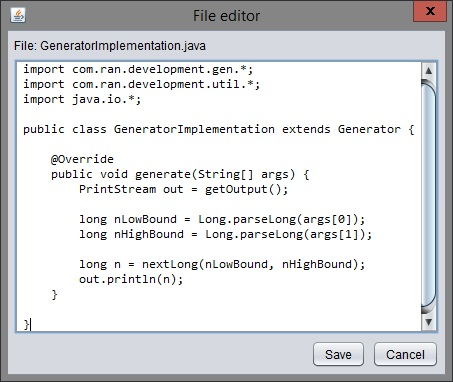
\includegraphics[scale=1.0]{screen_generator_code}}
\caption{Код генератора}
\label{screen_generator_code}
\end{figure}

\begin{figure}[!p]
\center{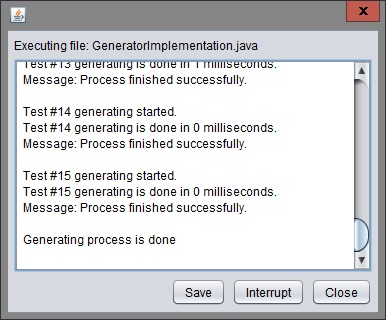
\includegraphics[scale=1.0]{screen_generator_result}}
\caption{Результаты запуска генератора}
\label{screen_generator_result}
\end{figure}

Чтобы просмотреть список прикреплённых к задаче валидаторов, нужно перейти на вкладку <<Validators>>. Здесь так же можно добавить и удалить валидатор, открыть его для редактирования или запустить, указав группу тестов для валидации (или специальный пункт <<All tests>>) и строковые параметры запуска. Данная вкладка отображена на рис.~\ref{screen_validators}. Для данной задачи валидатор также прост: происходит проверка принадлежности числа $n$ диапазону от 2 до $10^{12}$.

На вкладке <<Checkers>> (рис.~\ref{screen_checkers}) можно выбрать тип чекера, используемого при проверке решения данной задачи: либо чекер по умолчанию (<<Matching with the answer>>), либо специальный чекер с написанным для него кодом (<<Special checker>>). Поскольку к одной задаче можно прикрепить только один чекер, здесь не отображается список чекеров. Также отсюда можно открыть окно для редактирования кода чекера и попробовать перекомпилировать его, чтобы удостовериться, что код написан корректно.

\begin{figure}[!h]
\center{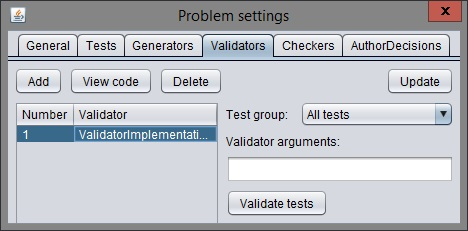
\includegraphics[scale=0.9]{screen_validators}}
\caption{Указание параметров запуска валидатора}
\label{screen_validators}
\end{figure}

\begin{figure}[!h]
\center{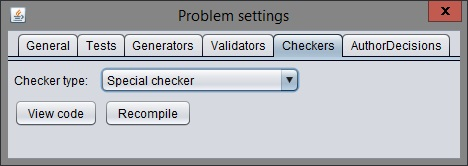
\includegraphics[scale=0.9]{screen_checkers}}
\caption{Указание типа чекера}
\label{screen_checkers}
\end{figure}

Чекер, используемый в данной задаче, выполняет следующие действия. Если участник вывел -1, чекер проверяет, что в ответе жюри тоже находится -1. Если же участник вывел целое число в интервале от 2 до $n$, проверяется, является ли это число множителем $n$.

\begin{figure}[!ht]
\center{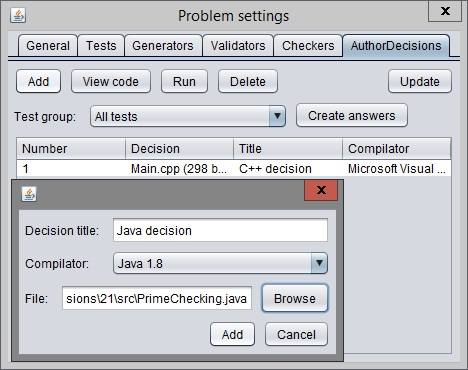
\includegraphics[scale=0.9]{screen_author_decisions}}
\caption{Добавление нового авторского решения}
\label{screen_author_decisions}
\end{figure}

На вкладке <<Author decisions>> можно просмотреть список авторских решений, прикреплённых к задаче (рис.~\ref{screen_author_decisions}). Здесь можно добавить новое решение (при этом отображается маленькое окно для ввода названия решения и выбора компилятора и файла с исходным кодом), удалить решение, открыть его код или запустить, чтобы увидеть вердикт на каждом тесте задачи. Кроме того, кнопка <<Create answers>> запускает генерацию ответов жюри (на каждом тесте из определённой группы, либо на тестах из всех групп, если выбран пункт <<All tests>>).

Главная идея авторского решения состоит в том, чтобы перечислять не все числа от 2 до $n$ для проверки, являются ли они множителем $n$, а только числа от 2 до $\sqrt{n}$, что, очевидно, происходит гораздо быстрее. Решение данной задачи на языке C++ состоит всего из одной функции \texttt{main()}, код которой выглядит следующим образом.

{\small
\begin{verbatim}
long long n;
cin >> n;

int s = (int)ceil(sqrt((double)n));
for (int i = 2; i <= s; i++) {
    if (i != n && n % i == 0) {
        cout << i << endl;
        return 0;
    }
}

cout << -1 << endl;
return 0;
\end{verbatim}
}

\begin{figure}[!b]
\center{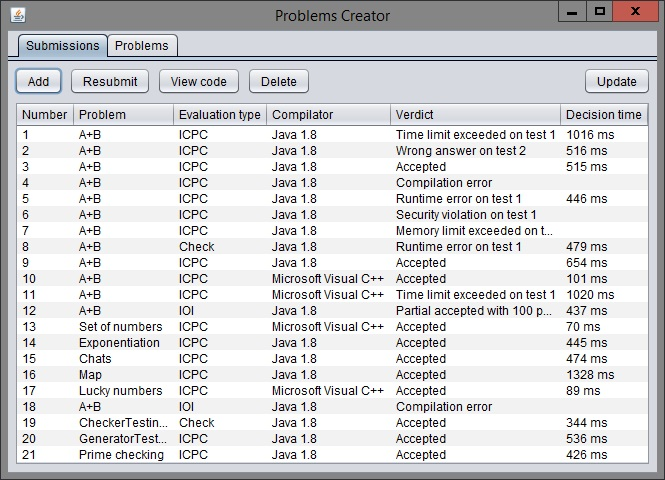
\includegraphics[scale=0.9]{screen_submissions}}
\caption{Список отправленных посылок}
\label{screen_submissions}
\end{figure}

\begin{figure}[!b]
\center{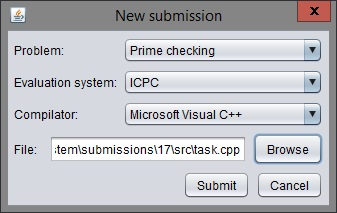
\includegraphics[scale=0.9]{screen_new_submission}}
\caption{Выбор параметров новой посылки}
\label{screen_new_submission}
\end{figure}

Рассмотрим теперь вторую вкладку главного окна приложения (рис.~\ref{screen_submissions}), на которой располагается список всех сохранённых в файловой системе посылок с вердиктами по каждой из них. Здесь можно добавить новую посылку, при этом открывается новое окно, отображённое на рис.~\ref{screen_new_submission}, в котором можно выбрать задачу, компилятор, систему оценивания и файл с исходный кодом. Также на данной вкладке можно удалить посылку, открыть её код для просмотра и перезапустить.

Мы сделаем посылку с решением, написанным на языке Java, но отличающимся от предыдущего рассмотренного решения в способе вывода множителя числа $n$. Если в прошлый раз мы выводили первое найденное число $i$, на которое $n$ делится нацело, то теперь мы будем выводить $n/i$. Ответ всё равно останется правильным, но во многих случаях окажется другим.

Запустим посылку и увидим окно, отображённое на рис.~\ref{screen_submission_results}, где видны вердикт и затраченное время по каждому тесту в задаче. Как можно видеть, такое решение также даёт вердикт <<Accepted>> на всех тестах, что говорит о корректной работе написанного нами чекера.

\begin{figure}[!h]
\center{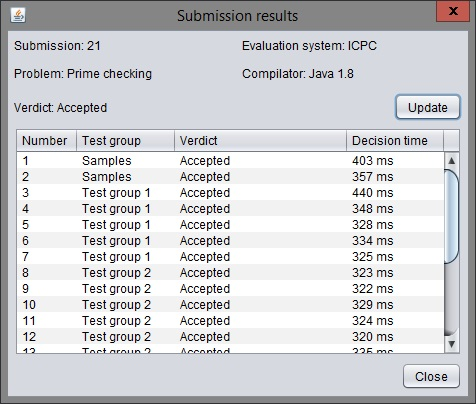
\includegraphics[scale=0.9]{screen_submission_results}}
\caption{Результаты запуска посылки на каждом тесте}
\label{screen_submission_results}
\end{figure}

\chapter*{Заключение}
\addcontentsline{toc}{chapter}{Заключение}
В данной работе была поставлена задача написать приложение для разработки задач по олимпиадному программированию и для тестирования решений. Предполагалось использование языка программирования Java и библиотеки компонентов графического интерфейса Swing.

Для решения поставленной задачи были рассмотрены основные принципы разработки задач и тестирования решений. Были описаны правила написания кода таких средств, как генераторы, валидаторы и чекеры, рассмотрены алгоритм тестирования посылки, различные системы оценивания и используемые вердикты, присуждаемые решениям.

Была спроектирована архитектура приложения, которое включило четыре модуля: библиотеку для разработки задач, а также модули для тестирования, доступа к файловой системе и взаимодействия с пользователем. Приложение было разработано, и практически все пакеты и классы, вошедшие в него, были подробно описаны. Наконец, был приведён пример работы приложения, описывающий процесс разработки простой задачи.

Ясно, что тематика, затронутая в данной работе, весьма актуальна сегодня, поэтому разработанное приложение вполне может найти себе применение, оказав большую помощь при подготовке тестов к задачам. Кроме того, функционал данного приложения возможно расширять и улучшать.

%В ходе курсовой работы было исследовано четыре различных алгоритма поиска выравниваний пар строк, обладающих определёнными характеристиками. Мы подробно обсудили, как используется в них принцип динамического программирования и каким образом строится искомое оптимальное выравнивание, поговорили об эффективности каждого из этих алгоритмов, а также дополнительно для двух из них выявили способ нахождения количества кооптимальных выравниваний.

%Была поставлена задача написать приложение, реализующее все четыре алгоритма и позволяющее запускать их с некоторым набором входных параметров. В ходе работы это приложение было разработано, в процессе чего активно использовались объектно-ориентированное программирование и паттерны проектирования. Была подробно описана структура классов, использованных в приложении, и приведён пример его работы.

%Ясно, что в созданном приложении реализованы лишь некоторые алгоритмы, работающие с выравниваниями строковых последовательностей, и что помимо них существует ещё множество подобных алгоритмов, из чего следует возможность дальнейшей разработки данного приложения.

\renewcommand{\bibname}{Список использованных источников}
\begin{thebibliography}{9}
\addcontentsline{toc}{chapter}{Список использованных источников}
\bibitem{wiki} Олимпиады по программированию // Википедия.~"--- URL: https://ru. wikipedia.org/wiki/Олимпиады\_по\_программированию (дата обращения: 02.05.2016).
\bibitem{ioi} Международная олимпиада по информатике // Википедия.~"--- URL: https:// ru.wikipedia.org/wiki/Международная\_олимпиада\_по\_информатике (дата обращения: 02.05.2016).
\bibitem{icpc} Международная студенческая олимпиада по программированию // Википедия.~"--- URL: https://ru.wikipedia.org/wiki/Международная\_студенческая\_ олимпиада\_по\_про\-грам\-ми\-рованию (дата обращения: 02.05.2016).
\bibitem{polygon} Платформа Polygon.~"--- URL: https://polygon.codeforces.com/ (дата обращения: 08.02.2016).
\bibitem{codeforces} Платформа Codeforces.~"--- URL: http://codeforces.com/ (дата обращения: 08.02.2016).
\bibitem{gamma} Приёмы объектно-ориентированного проектирования. Паттерны проектирования~/ Э. Гамма [и др.].~"--- Санкт-Петербург: Питер, 2001.~"--- 368 с.
\bibitem{java} Java Platform Standard Edition 8 Documentation.~"--- URL: http:// docs.oracle.com/javase/8/docs/ (дата обращения: 15.03.2016).
\bibitem{testlib} Testlib // Codeforces.~"--- URL: http://codeforces.com/testlib (дата обращения: 11.04.2016).
\bibitem{cornell2} Хорстманн К.С. Java. Библиотека профессионала, том 2. Расширенные средства~/ К.С. Хорстманн, Г. Корнелл; пер. с англ. и ред. И.В.Берштейна.~"--- 9-е изд.~"--- Москва: ООО~<<И.Д.~Вильямс>>, 2014.~"--- 1008 с.
%\bibitem{cornell1} Хорстманн Кей С. Java. Библиотека профессионала, том 1. Основы~/ Кей С. Хорстманн, Гари Корнелл; пер. с англ. и ред. И.В.Берштейна.~"--- 9-е изд.~"--- Москва: ООО~<<И.Д.~Вильямс>>, 2014.~"--- 864 с.
\end{thebibliography}

\newpage
\appendix
\addtocontents{toc}{\vspace{5mm}\bfseries Приложения\par}
\footnotesize
\chapter{Библиотека для разработки задач}
\section*{\texttt{Generator.java}}
\begin{verbatim}
package com.ran.development.gen;

// Импорт классов
// ...

public abstract class Generator {

    private static final long DEFAULT_RANDOM_SEED = 1938572538L;
    
    public static Generator getDefault() {
        return new Generator() {
            @Override
            protected void generate(String[] args) { }
        };
    }
    
    // Генератор псевдослучайных чисел
    private Random random;
    // Поток вывода в файл
    private PrintStream output;
    // Парсер регулярных выражений
    private RegularExpressionParser parser = new RegularExpressionParser();
    
    // Контструкторы, геттеры, сеттеры
    // ...
    
    // print-методы
    // ...
    
    protected int nextInt(int higherBound) {
        return random.nextInt(higherBound);
    }
    
    protected int nextInt(int lowerBound, int higherBound) {
        return lowerBound + random.nextInt(higherBound - lowerBound + 1);
    }
    
    // Ещё next-методы
    // ...
    
    protected int any(int[] values) {
        return values[random.nextInt(values.length)];
    }
    
    protected char any(String regularExpression) {
        int quantity = parser.getCharactersQuantity(regularExpression);
        return parser.getCharacter(regularExpression, random.nextInt(quantity));
    }
    
    // Ещё any-методы
    // ...
    
    // Метод непосредственной генерации входных данных
    abstract protected void generate(String[] args);
    
}
\end{verbatim}

\section*{\texttt{MultiGenerator.java}}
\begin{verbatim}
package com.ran.development.gen;

// Импорт классов
// ...

public class MultiGenerator {
    
    private static final long MESSAGING_DELAY = 2000;
    
    // Набор слушателей процесса генерации
    private DevelopmentListenerSupport listenerSupport = new DevelopmentListenerSupport();
    // Поставщик генератора
    private Supplier<? extends Generator> generatorSupplier = () -> {
        return Generator.getDefault();
    };
    // Инициализирующее значение генератора псевдослучайных чисел
    private int randomSeed = 0;
    // Пути файлов для генерации входных данных
    private Path[] paths = { };
    // Аргументы запуска генератора
    private String[] arguments = { };
    
    // Геттеры, сеттеры, методы работы со слушателями
    // ...
    
    // Запуск генератора в отдельном потоке
    public void performGenerating() {
        listenerSupport.fireProcessingStarted();
        Generator generator = generatorSupplier.get();
        if (generator == null) {
            finishEarlier("Cannot instantiate Generator subclass",
                    DevelopmentResult.FAIL, 1, paths.length);
            return;
        }
        generator.setRandomSeed(randomSeed);
        for (int index = 1; index <= paths.length; index++) {
            listenerSupport.fireTaskProcessingStarted(index);
            Path path = paths[index - 1];
            long start = System.currentTimeMillis();
            Thread thread = null;
            try (OutputStream output = Files.newOutputStream(path)) {
                generator.setOutput(output);
                FutureTask<DevelopmentResult> futureTask = new FutureTask<>(
                        new GeneratingTask(generator, index, arguments));
                thread = new Thread(futureTask);
                start = System.currentTimeMillis();
                thread.start();
                while (thread.isAlive()) {
                    thread.join(MESSAGING_DELAY);
                    if (thread.isAlive()) {
                        listenerSupport.fireTaskIsProcessing(index,
                                System.currentTimeMillis() - start);
                    }
                }
                listenerSupport.fireTaskIsDone(futureTask.get());
            } // Перехват исключений, вывод в лог
            // ...
        }
        listenerSupport.fireProcessingFinished();
    }
    
    // Вспомогательные методы
    // ...
    
    // Задача запуска генератора
    private static class GeneratingTask implements Callable<DevelopmentResult> {
        private String[] arguments;
        private Generator generator;
        private int generatorNumber;
        
        // Конструктор
        // ...
        
        @Override
        public DevelopmentResult call() {
            long start = System.currentTimeMillis();
            try {
                generator.generate(arguments);
            } // Перехват исключений, вывод в лог
            // ...
            return new DevelopmentResult(generatorNumber, System.currentTimeMillis() - start);
        }
    }
    
}
\end{verbatim}

\section*{\texttt{Validator.java}}
\begin{verbatim}
package com.ran.development.valid;

// Импорт классов
// ...

public abstract class Validator {

    public static Validator getDefault() {
        return new Validator() {
            @Override
            public void validate(String[] args) throws ValidationException { }
        };
    }
    
    // Строгий ввод валидируемых входных данных
    private StrictInput input = StrictInput.getEmptyInput();
    // Парсер регулярных выражений
    private RegularExpressionParser parser = new RegularExpressionParser();

    // Конструкторы, геттеры, сеттеры
    // ...
    
    protected void error() throws ValidationException {
        throw new ValidationException(input.getState());
    }
    
    protected void error(String message) throws ValidationException {
        throw new ValidationException(message, input.getState());
    }
    
    protected void ensure(boolean condition) throws ValidationException {
        if (!condition) {
            error("Condition is not true");
        }
    }
    
    protected void inBounds(int lowEdge, int number, int highEdge)
            throws ValidationException {
        if (!(lowEdge <= number && number <= highEdge)) {
            error("Number out of bounds");
        }
    }
    
    // Ещё inBounds-методы
    // ...
    
    protected void matchesExpression(char symbol, String regularExpression)
            throws ValidationException {
        if (!parser.matchesExpression(symbol, regularExpression)) {
            error("Symbol does not match the regular expression");
        }
    }
    
    // Ещё matchesExpression-методы
    // ...
    
    protected void inValues(int number, int[] values) throws ValidationException {
        for (int value: values) {
            if (value == number) {
                return;
            }
        }
        error("Number is not in values array");
    }
    
    // Ещё inValues-методы
    // ...
    
    // Метод-обёртка для проверки, что файл прочитал полностью
    public void performValidation(String[] args) throws ValidationException {
        validate(args);
        if (!input.isReaden()) {
            error("File was not readen completely");
        }
    }
    
    // Метод непосредственной валидации входных данных
    public abstract void validate(String[] args) throws ValidationException;
    
}
\end{verbatim}

\section*{\texttt{Checker.java}}
\begin{verbatim}
package com.ran.development.check;

// Импорт классов
// ...

public abstract class Checker {

    public static final int OK = 0,
            WRONG_ANSWER = 1,
            FAIL = 2;

    // Лексемный ввод входных данных
    private TokenInput input = TokenInput.getEmptyInput();
    // Лексемный ввод ответа участника
    private TokenInput output = TokenInput.getEmptyInput();
    // Лексемный ввод ответа жюри
    private TokenInput answer = TokenInput.getEmptyInput();
    // Парсер регулярных выражений
    private RegularExpressionParser parser = new RegularExpressionParser();

    // Геттеры, сеттеры
    // ...

    protected void quit(int resultInfo, String message) throws CheckResultException {
        throw new CheckResultException(resultInfo, message);
    }

    // Ещё quit-методы
    // ...

    protected void quitIf(boolean condition, int resultInfo, String message)
            throws CheckResultException {
        if (condition) {
            quit(resultInfo, message);
        }
    }

    // Ещё quitIf-методы
    // ...

    protected void ensureIf(boolean condition, String message) throws CheckResultException {
        if (!condition) {
            quit(WRONG_ANSWER, message);
        }
    }

    // Ещё ensureIf-методы
    // ...

    // Метод-обёртка для перехвата исключения
    public void performChecking() throws CheckResultException {
        try {
            check();
        } catch (CheckResultException exception) {
            if (exception.getResultInfo() == OK && !output.checkEof()) {
                quit(WRONG_ANSWER, "Extra values in the output");
            }
            throw exception;
        }
        quit(FAIL, "Checker did not tell result of checking");
    }

    // Метод непосредственной проверки ответа
    public abstract void check() throws CheckResultException;

}
\end{verbatim}

\section*{\texttt{Utils.java}}
\begin{verbatim}
package com.ran.development.util;

// Импорт классов
// ...

// Класс для динамической загрузки классов
public class Utils {

    private Utils() { }
    
    public static <T> Supplier<? extends T> getSupplier(Class<T> parentClass,
            Path classFilePath) {
        try {
            Path folderPath = classFilePath.getParent();
            String className = getClassName(classFilePath);
            ClassLoader loader = new URLClassLoader(new URL[] { folderPath.toUri().toURL() });
            Class<? extends T> cl = (Class<? extends T>)loader.loadClass(className);
            cl.newInstance();
            return () -> {
                try {
                    return cl.newInstance();
                } catch (InstantiationException | IllegalAccessException exception) {
                    String message = "Cannot create instance of " + parentClass.getName() +
                            " subclass";
                    DevelopmentLogging.logger.log(Level.FINE, message, exception);
                    return null;
                }
            };
        } // Перехват исключений, вывод в лог
        // ...
    }
    
    // Вспомогательные методы
    // ...
    
}
\end{verbatim}
\chapter{Тестирующий модуль}
\section*{\texttt{TestingSystem.java}}
\begin{verbatim}
package com.ran.testing.system;

// Интерфейс ядра тестирующей системы
public interface TestingSystem {
    
    public void start();
    public void addSubmission(TestingInfo info);
    public void stop();
    
}
\end{verbatim}

\section*{\texttt{MultithreadTestingSystem.java}}
\begin{verbatim}
package com.ran.testing.system;

// Импорт классов
// ...

// Реализация ядра тестирующей системы, работающая во многих потоках
public class MultithreadTestingSystem implements TestingSystem {

    private static final int DEFAULT_THREADS_QUANTITY = Runtime.getRuntime()
            .availableProcessors();
    private static MultithreadTestingSystem defaultSystem = null;
    
    public static MultithreadTestingSystem getDefault() {
        if (defaultSystem == null) {
            defaultSystem = new MultithreadTestingSystem(DEFAULT_THREADS_QUANTITY);
        }
        return defaultSystem;
    }
    
    // Максимальное количество используемых потоков
    private int threadsQuantity;
    // Поставщик временных и конфигурационных файлов
    private TestingFileSupplier fileSupplier;
    private ExecutorService service;
    private ExecutorCompletionService<TestingInfo> completionService;
    // Счётчик текущего количества проверяемых посылок
    private int submissionsCounter = 0;
    // Поток для обработки результатов проверки
    private Thread resultHandlersThread;

    // Конструкторы, геттеры, сеттеры
    // Синхронизованные методы обновления счётчика проверяемых посылок
    // ...
    
    // Инициализация и старт ядра тестирующей системы
    @Override
    public void start() {
        service = Executors.newFixedThreadPool(threadsQuantity);
        completionService = new ExecutorCompletionService<>(service);
        resultHandlersThread = new Thread(new ResultTracking());
        resultHandlersThread.start();
    }

    // Добавление новой посылки на проверку
    @Override
    public void addSubmission(TestingInfo info) {
        submissionsCounterUp();
        completionService.submit(new TestingTask(info, fileSupplier));
    }

    // Остановка ядра тестирующей системы
    @Override
    public void stop() {
        service.shutdown();
        resultHandlersThread.interrupt();
    }
    
    // Процесс обработки результатов проверки очередной посылки
    // Выполняется в отдельном потоке
    private class ResultTracking implements Runnable {
        public void run() {
            boolean interrupted = false;
            while (!interrupted || getSubmissionsCounter() > 0) {
                try {
                    Future<TestingInfo> future = completionService.take();
                    submissionsCounterDown();
                    TestingInfo info = future.get();
                    info.getTestResultHandler().process(info);
                } // Перехват исключений, вывод в лог
                // ...
            }
        }
    }
    
    // Задача тестирования одной посылки
    private static class TestingTask implements Callable<TestingInfo> {
        private TestingInfo info;
        private TestingFileSupplier fileSupplier;
        // Конструктор
        // ...
        public TestingInfo call() {
            info.getProblemTester().performTesting(fileSupplier, info);
            return info;
        }
    }
    
}
\end{verbatim}

\section*{\texttt{Verdict.java}}
\begin{verbatim}
package com.ran.testing.system;

// Виды вердиктов по посылке или тесту
public enum Verdict {

    NOT_TESTED,
    WAITING,
    TESTING,
    ACCEPTED,
    PRETESTS_ACC,
    PARTIAL_ACC,
    COMPILE_ERROR,
    RUNTIME_ERROR,
    WRONG_ANSWER,
    TIME_LIMIT,
    MEMORY_LIMIT,
    SECUR_VIOL,
    FAIL

}
\end{verbatim}

\section*{\texttt{VerdictInfo.java}}
\begin{verbatim}
package com.ran.testing.system;

// Полная информация о результате тестирования
public class VerdictInfo implements Cloneable {

    public static final VerdictInfo VERDICT_NOT_TESTED = new VerdictInfo(Verdict.NOT_TESTED);
    public static final VerdictInfo VERDICT_COMPILE_ERROR = new VerdictInfo(Verdict.COMPILE_ERROR);
    public static final VerdictInfo VERDICT_MEMORY_LIMIT = new VerdictInfo(Verdict.MEMORY_LIMIT);
    public static final VerdictInfo VERDICT_SECUR_VIOL = new VerdictInfo(Verdict.SECUR_VIOL);
    public static final VerdictInfo VERDICT_FAIL = new VerdictInfo(Verdict.FAIL);

    private Verdict verdict;
    private Integer decisionTime;
    private Short decisionMemory;
    private Short points;
    private Integer wrongTestNumber;

    // Конструкторы, геттеры, сеттеры
    // ...

    @Override
    public VerdictInfo clone() {
        return new VerdictInfo(this.verdict, this.points)
                .setDecisionTime(this.decisionTime)
                .setDecisionMemory(this.decisionMemory)
                .setWrongTestNumber(this.wrongTestNumber);
    }

}
\end{verbatim}

\section*{\texttt{TestingInfo.java}}
\begin{verbatim}
package com.ran.testing.system;

// Импорт классов
// ...

// Полная информация о том, как нужно тестировать очередную посылку
public class TestingInfo {

    // Обработчик результатов проверки посылки
    private TestResultHandler testResultHandler;
    // Алгоритм проверки посылки
    private ProblemTester problemTester;
    // Система оценивания
    private EvaluationSystem evaluationSystem;
    // Инструментарий языка программирования
    private LanguageToolkit languageToolkit;
    // Способ проверки корректности ответа по тесту
    private Checker checker;
    // Поставщик файлов с исходным кодом и скомпилированным файлом
    private CodeFileSupplier codeFileSupplier;
    // Поставщик файлов с тестами
    private ProblemFileSupplier problemFileSupplier;
    // Необходимость тестировать только на претестах
    private boolean pretestsOnly;
    // Ограничение по времени
    private Integer timeLimit;
    // Ограничение по памяти
    private Short memoryLimit;
    // Таблица с полной информацией о тестах из каждой группы
    private TestTable testTable;
    // Результаты тестирования посылки
    private VerdictInfo verdictInfo = null;

    // Конструктор, геттеры, сеттеры
    // ...

}
\end{verbatim}

\section*{\texttt{ProblemTester.java}}
\begin{verbatim}
package com.ran.testing.tester;

// Импорт классов
// ...

// Алгоритм тестирования посылки
public interface ProblemTester {

    void performTesting(TestingFileSupplier fileSupplier, TestingInfo info);

}
\end{verbatim}

\section*{\texttt{EvaluationSystem.java}}
\begin{verbatim}
package com.ran.testing.evaluation;

// Импорт классов
// ...

public interface EvaluationSystem {

    void orderTesting(TesterDelegate delegate, boolean pretestsOnly);
    VerdictInfo getVerdictInfo(TestTable testTable, boolean pretestsOnly);
    ProblemResult countProblemResult(TreeMap<Date, VerdictInfo> verdictsMap,
            Date competitionBeginning);

    // Интерфейс делегата для доступа к запуску тестирования
    public interface TesterDelegate {
        TestTable getTestTable();
        Integer performTestGroup(TestGroupType type, boolean upToFirstFailure);
        VerdictInfo performOneTest(TestGroupType type, int testNumber);
    }
    
    // Результат по определённой задаче
    public class ProblemResult {
        private short points;
        private int fine;
        // Конструктор, геттеры, сеттеры
        // ...
    }

}
\end{verbatim}

\section*{\texttt{LanguageToolkit.java}}
\begin{verbatim}
package com.ran.testing.language;

// Импорт классов
// ...

// Инструментарий языка программирования
public interface LanguageToolkit {
    
    int compile(Path sourceFile, Path compileFolder, Path configFolder) throws FailException;
    int compile(Path sourceFile, Path compileFolder, Path configFolder,
            OutputStream errorStream) throws FailException;
    ExecutionInfo execute(Path compileFile, Path inputFile, Path outputFile,
            Path configFolder, int timeLimit, short memoryLimit)
            throws FailException, TimeLimitException, MemoryLimitException,
            SecurityViolatedException;

    // Результат запуска программы
    public class ExecutionInfo {
        private int exitCode;
        private Integer decisionTime;
        private Short decisionMemory;
        // Конструктор, геттеры
        // ...
    }
    
    static final OutputStream EMPTY_OUTPUT_STREAM = new OutputStream() {
        @Override
        public void write(int b) throws IOException {
        }
    };
    
}
\end{verbatim}

\section*{\texttt{JavaLanguageToolkit.java}}
\begin{verbatim}
package com.ran.testing.language;

// Импорт классов
// ...

// Инструментарий для языка Java
public class JavaLanguageToolkit implements LanguageToolkit {
    
    private static final String POLICY_FILE_NAME = "java_problem.policy";
    private static final String PROPERTIES_FILE_NAME = "java.properties";
    private static final String JAVA_PATH_PROPERTY = "java_path";
    private static final String STACK_SIZE_PROPERTY = "stack_size";
    
    // Другие статические константы
    // ...
    
    private static Properties javaProperties = null;
    private static Path javaPropertiesLocation = null;
    
    // Метод доступа к заданным свойствам инструментария Java
    private static Properties getJavaProperties(Path configFolder) throws FailException {
        if (javaProperties == null || !Objects.equals(configFolder, javaPropertiesLocation)) {
            javaProperties = new Properties();
            try {
                javaProperties.load(Files.newInputStream(
                        configFolder.resolve(PROPERTIES_FILE_NAME)));
            } catch (IOException exception) {
                throw new FailException("Fail because of exception while loading "
                        + PROPERTIES_FILE_NAME, exception);
            }
            javaPropertiesLocation = configFolder;
        }
        return javaProperties;
    }
    
    // Компиляция программы на Java (без вывода ошибок)
    @Override
    public int compile(Path sourceFile, Path compileFolder, Path configFolder)
            throws FailException {
        return compile(sourceFile, compileFolder, configFolder, EMPTY_OUTPUT_STREAM);
    }

    // Компиляция программы на Java (с выводом ошибок)
    @Override
    public int compile(Path sourceFile, Path compileFolder, Path configFolder,
            OutputStream errorStream) throws FailException {
        if (Files.notExists(sourceFile) || Files.notExists(compileFolder)) {
            throw new FailException("Compilation failed because files were not found.");
        }
        JavaCompiler compiler = ToolProvider.getSystemJavaCompiler();
        return compiler.run(null, null, errorStream, "-d", compileFolder.toString(),
                sourceFile.toString());
    }

    // Запуск программы на Java
    @Override
    public ExecutionInfo execute(Path compileFile, Path inputFile, Path outputFile,
            Path configFolder, int timeLimit, short memoryLimit)
            throws FailException, TimeLimitException, MemoryLimitException,
            SecurityViolatedException {
        Properties javaProperties = getJavaProperties(configFolder);
        String javaPathProperty = javaProperties.getProperty(JAVA_PATH_PROPERTY);
        String stackSizeProperty = javaProperties.getProperty(STACK_SIZE_PROPERTY);
        Path policyPath = configFolder.resolve(POLICY_FILE_NAME);
        if (Files.notExists(compileFile) || Files.notExists(inputFile) ||
                Files.notExists(outputFile) || Files.notExists(policyPath) ||
                javaPathProperty == null || stackSizeProperty == null) {
            throw new FailException("Execution failed because files or properties were not found.");
        }
        try {
            Path javaPath = Paths.get(javaPathProperty);
            String memoryOption = "-Xmx" + memoryLimit + "M";
            String stackOption = "-Xss" + stackSizeProperty + "M";
            String managerOption = "-Djava.security.manager";
            String policyOption = "-Djava.security.policy==" + policyPath.toString();
            String className = getClassName(compileFile);
            ProcessBuilder processBuilder = new ProcessBuilder("\"" + javaPath.toString() + "\"",
                    memoryOption, stackOption, managerOption, policyOption, className);
            Path compileFolder = compileFile.getParent();
            processBuilder.directory(compileFolder.toFile());
            processBuilder.redirectInput(inputFile.toFile());
            processBuilder.redirectOutput(outputFile.toFile());
            Process process = null;
            try {
                long start = System.currentTimeMillis();
                process = processBuilder.start();
                process.waitFor(timeLimit, TimeUnit.MILLISECONDS);
                int decisionTime = (int)(System.currentTimeMillis() - start);
                if (process.isAlive()) {
                    throw new TimeLimitException(decisionTime);
                }
                int exitValue = process.exitValue();
                if (exitValue != 0) {
                    analyseErrorStream(process.getErrorStream());
                }
                return new ExecutionInfo(exitValue, decisionTime, null);
            } finally {
                if (process != null) {
                    process.destroyForcibly();
                    process.waitFor();
                }
            }
        } catch (InterruptedException | IOException exception) {
            throw new FailException(
                    "InterruptedException or IOException while execution.", exception);
        }
    }
    
    // Вспомогательные методы
    // ...

}
\end{verbatim}

\section*{\texttt{Checker.java}}
\begin{verbatim}
package com.ran.testing.checker;

// Импорт классов
// ...

// Способ проверки корректности ответа
public interface Checker {

    default void initialize(ProblemFileSupplier problemFileSupplier) { }
    Verdict check(Path inputPath, Path outputPath, Path answerPath);

}
\end{verbatim}
\chapter{Модуль для работы с файловой системой}
Модуль для работы с файловой системой (код).
\chapter{Модуль с графическим интерфейсом}
\section*{\texttt{Main.java}}
\begin{verbatim}
package com.ran.interaction.main;

// Импорт классов
// ...

public class Main {

    // Подключение класса специального чекера
    private static void plugInClasses() {
        JavaClassChecker.plugInClass();
    }

    // Запуск главного контроллера
    public static void main(String[] args) {
        plugInClasses();
        MainController controller = new MainController();
        controller.init();
        controller.showFrame();
    }

}
\end{verbatim}

\section*{\texttt{Observer.java}}
\begin{verbatim}
package com.ran.interaction.observer;

// Интерфейс наблюдателя
@FunctionalInterface
public interface Observer {

    // Метод для оповещения наблюдателя
    void notify(String id, Object parameter);
    
}
\end{verbatim}

\section*{\texttt{Publisher.java}}
\begin{verbatim}
package com.ran.interaction.observer;

import java.util.List;

// Интерфейс издателя
public interface Publisher {

    // Метод доступа к списку доступных идентификаторов событий
    List<String> getAvailableIds();
    // Метод подписки наблюдателя к определённому событию
    void subscribe(String id, Observer observer);
    Observer getObserver(String id);
    
    // Метод инициализации наблюдателей по умолчанию
    default void initObservers() {
        for (String id: getAvailableIds()) {
            subscribe(id, EmptyObserver.getInstanse());
        }
    }
    
    // Метод оповещения наблюдателей об определённом событии
    default void notifyObservers(Object parameter) {
        for (String id: getAvailableIds()) {
            getObserver(id).notify(id, parameter);
        }
    }
    
}
\end{verbatim}

\section*{\texttt{MainFrame.java}}
\begin{verbatim}
package com.ran.interaction.windows;

// Импорт классов
// ...

// Главное окно приложения
public class MainFrame extends JFrame {

    private static final String SUBMISSIONS = "Submissions";
    private static final String PROBLEMS = "Problems";
    
    public MainFrame() {
        setDefaultCloseOperation(JFrame.EXIT_ON_CLOSE);
        initComponents();
        initCustomComponents();
    }

    // Код создания интерфейса окна, поля с компонентами
    // ...

    private SubmissionsPanel submissionsPanel;
    private ProblemsPanel problemsPanel;

    private void initCustomComponents() {
        submissionsPanel = new SubmissionsPanel();
        tabbedPane.add(submissionsPanel);
        tabbedPane.setTitleAt(0, SUBMISSIONS);
        problemsPanel = new ProblemsPanel();
        tabbedPane.add(problemsPanel);
        tabbedPane.setTitleAt(1, PROBLEMS);
    }
    
    public SubmissionsPanel getSubmissionsPanel() {
        return submissionsPanel;
    }

    public ProblemsPanel getProblemsPanel() {
        return problemsPanel;
    }
    
}
\end{verbatim}

\section*{\texttt{SubmissionsPanel.java}}
\begin{verbatim}
package com.ran.interaction.panels;

// Импорт классов
// ...

// Панель с посылками
public class SubmissionsPanel extends JPanel implements Publisher {

    // Идентификаторы событий панели
    public static final String ADD = "add_submission";
    public static final String RESUBMIT = "resubmit_submission";
    public static final String DELETE = "delete_submission";
    public static final String UPDATE = "update_submissions";
    public static final String VIEW_CODE = "view_submission_code";
    
    // Дополнительные статические константы
    // ...
    
    public SubmissionsPanel() {
        initComponents();
        initCustomComponents();
        setTableContent(new Object[][] { });
        initObservers();
    }

    // Код создания интерфейса окна, поля с компонентами 
    // ...                    

    // Набор зарегистрированных наблюдателей
    private Map<String, Observer> observers = new HashMap<>();
    
    // Настройка механизма оповещения наблюдателей о событиях
    private void initCustomComponents() {
        buttonAdd.addActionListener(event -> getObserver(ADD).notify(ADD, null));
        buttonResubmit.addActionListener(event -> callObserverIfRowIsSelected(RESUBMIT));
        buttonDelete.addActionListener(event -> callObserverIfRowIsSelected(DELETE));
        buttonViewCode.addActionListener(event -> callObserverIfRowIsSelected(VIEW_CODE));
        buttonUpdate.addActionListener(event -> getObserver(UPDATE).notify(UPDATE, null));
    }
    
    private void callObserverIfRowIsSelected(String id) {
        if (tableSubmissions.getSelectedIdentifier() != null) {
            getObserver(id).notify(id, tableSubmissions.getSelectedIdentifier());
        }
    }
    
    @Override
    public List<String> getAvailableIds() {
        return Arrays.asList(ADD, RESUBMIT, DELETE, VIEW_CODE, UPDATE);
    }
    
    @Override
    public void subscribe(String id, Observer observer) {
        observers.put(id, observer);
    }

    @Override
    public Observer getObserver(String id) {
        return observers.getOrDefault(id, EmptyObserver.getInstanse());
    }
    
    public final void setTableContent(Object[][] content) {
        tableSubmissions.setTableContent(content, TABLE_HEADERS);
    }
    
}
\end{verbatim}

\section*{\texttt{ProblemsPanel.java}}
\begin{verbatim}
package com.ran.interaction.panels;

// Импорт классов
// ...

// Панель с задачами
public class ProblemsPanel extends JPanel implements Publisher {
    
    // Идентификаторы событий панели
    public static final String ADD = "add_problem";
    public static final String EDIT = "edit_problem";
    public static final String DELETE = "delete_problem";
    public static final String UPDATE = "update_problems";
    
    // Дополнительные статические константы
    // ...
    
    public ProblemsPanel() {
        initComponents();
        initCustomComponents();
        setTableContent(new Object[][] { });
        initObservers();
    }

    // Код создания интерфейса окна, поля с компонентами
    // ...

    // Набор зарегистрированных наблюдателей
    private Map<String, Observer> observers = new HashMap<>();
    
    // Настройка механизма оповещения наблюдателей о событиях
    private void initCustomComponents() {
        buttonAdd.addActionListener(event -> getObserver(ADD).notify(ADD, null));
        buttonEdit.addActionListener(event -> callObserverIfRowIsSelected(EDIT));
        buttonDelete.addActionListener(event -> callObserverIfRowIsSelected(DELETE));
        buttonUpdate.addActionListener(event -> getObserver(UPDATE).notify(UPDATE, null));
    }
    
    private void callObserverIfRowIsSelected(String id) {
        if (tableProblems.getSelectedIdentifier() != null) {
            getObserver(id).notify(id, tableProblems.getSelectedIdentifier());
        }
    }
    
    @Override
    public List<String> getAvailableIds() {
        return Arrays.asList(ADD, EDIT, DELETE, UPDATE);
    }
    
    @Override
    public void subscribe(String id, Observer observer) {
        observers.put(id, observer);
    }

    @Override
    public Observer getObserver(String id) {
        return observers.getOrDefault(id, EmptyObserver.getInstanse());
    }
    
    public final void setTableContent(Object[][] content) {
        tableProblems.setTableContent(content, TABLE_HEADERS);
    }
    
}
\end{verbatim}

\section*{\texttt{MainController.java}}
\begin{verbatim}
package com.ran.interaction.controllers;

// Импорт классов
// ...

// Главный контроллер приложения
public class MainController {

    // Объединённые ядро тестирующей системы и поставщик файлов
    private ProblemsCreator creator;
    // Главное окно приложения
    private MainFrame mainFrame;

    public void init() {
        creator = new ProblemsCreator();
        creator.init();
    }
    
    public void showFrame() {
        EventQueue.invokeLater(() -> {
            try {
                for (UIManager.LookAndFeelInfo info : UIManager.getInstalledLookAndFeels()) {
                    if ("Nimbus".equals(info.getName())) {
                        UIManager.setLookAndFeel(info.getClassName());
                        break;
                    }
                }
            } catch (ClassNotFoundException | InstantiationException |
                    IllegalAccessException | UnsupportedLookAndFeelException exception) {
                InteractionLogging.logger.log(Level.FINE,
                        "Cannot set Nimbus Look and Feel", exception);
            }
            mainFrame = new MainFrame();
            configurateMainFrame(mainFrame);
            mainFrame.setVisible(true);
        });
    }

    // Настройка главного окна приложения
    // Подписка наблюдателей
    private void configurateMainFrame(MainFrame mainFrame) {
        mainFrame.addWindowListener(new WindowAdapter() {
            public void windowClosing(WindowEvent event) {
                creator.stop();
            }
        });
        SubmissionsPanel submissionsPanel = mainFrame.getSubmissionsPanel();
        updateSubmissions(null, null);
        submissionsPanel.subscribe(SubmissionsPanel.ADD, this::addSubmission);
        submissionsPanel.subscribe(SubmissionsPanel.RESUBMIT, this::submitSubmission);
        submissionsPanel.subscribe(SubmissionsPanel.VIEW_CODE, this::viewSubmissionCode);
        submissionsPanel.subscribe(SubmissionsPanel.DELETE, this::deleteSubmission);
        submissionsPanel.subscribe(SubmissionsPanel.UPDATE, this::updateSubmissions);
        ProblemsPanel problemsPanel = mainFrame.getProblemsPanel();
        updateProblems(null, null);
        problemsPanel.subscribe(ProblemsPanel.ADD, this::addProblem);
        problemsPanel.subscribe(ProblemsPanel.EDIT, this::editProblem);
        problemsPanel.subscribe(ProblemsPanel.DELETE, this::deleteProblem);
        problemsPanel.subscribe(ProblemsPanel.UPDATE, this::updateProblems);
    }
    
    // Обработчик события добавления новой посылки
    private void addSubmission(String id, Object parameter) {
        SubmissionCreationController creationController = new SubmissionCreationController();
        creationController.setFileSupplier(creator.getFileSupplier());
        creationController.showDialog();
        String submissionFolder = creationController.getSubmissionFolder();
        if (submissionFolder != null) {
            updateSubmissions(null, null);
            submitSubmission(null, submissionFolder);
        }
    }
    
    // Обработчик события запуска посылки
    private void submitSubmission(String id, Object parameter) {
        String submissionFolder = parameter.toString();
        SubmissionResultController resultController = new SubmissionResultController();
        resultController.setFileSupplier(creator.getFileSupplier());
        resultController.setTestingSystem(creator.getTestingSystem());
        resultController.setSubmissionFolder(submissionFolder);
        resultController.showDialog();
        updateSubmissions(null, null);
    }
    
    // Обработчик события просмотра кода посылки
    private void viewSubmissionCode(String id, Object parameter) {
        String submissionFolder = parameter.toString();
        Path sourceFilePath = creator.getFileSupplier()
                .getSubmissionCodeSupplier(submissionFolder).getSourceFile();
        FileEditorController editorController = new FileEditorController();
        editorController.showDialog(sourceFilePath, true);
    }
    
    // Обработчик события удаления посылки
    private void deleteSubmission(String id, Object parameter) {
        int answer = SwingUtil.showYesNoDialog(mainFrame,
                SubmissionsPanel.DELETING_MESSAGE, SubmissionsPanel.DELETING_TITLE);
        if (answer == JOptionPane.YES_OPTION) {
            creator.getFileSupplier().deleteSubmissionFolder(parameter.toString());
            updateSubmissions(null, null);
        }
    }
    
    // Обработчик события обновления посылок
    private void updateSubmissions(String id, Object parameter) {
        FileSupplier fileSupplier = creator.getFileSupplier();
        Properties properties = PresentationSupport.getPresentationProperties();
        List<String> submissionNumbers = fileSupplier.getSubmissionsFolderNames();
        Object[][] content = SwingUtil.prepareTableContent(submissionNumbers, (number, row) -> {
            row.add(number);
            SubmissionDescriptor descriptor = fileSupplier.getSubmissionDescriptor(number);
            String problemNumber = descriptor.getProblemName();
            row.add(fileSupplier.getProblemsFolderNames().contains(problemNumber) ?
                    fileSupplier.getProblemDescriptor(problemNumber).getProblemName() : "");
            row.add(properties.getProperty(descriptor.getEvaluationType()));
            row.add(properties.getProperty(descriptor.getCompilatorName()));
            row.add(TestingUtil.getVerdictDescription(descriptor.getVerdict(),
                    descriptor.getDecisionPoints(), descriptor.getWrongTestNumber()));
            row.add(TestingUtil.getTimeDescription(descriptor.getDecisionTime()));
        });
        mainFrame.getSubmissionsPanel().setTableContent(content);
    }
    
    // Обработчик события добавления задачи
    private void addProblem(String id, Object parameter) {
        creator.getFileSupplier().addProblemFolder();
        updateProblems(null, null);
    }
    
    // Обработчик события редактирования задачи
    private void editProblem(String id, Object parameter) {
        ProblemController problemController = new ProblemController();
        problemController.setFileSupplier(creator.getFileSupplier());
        problemController.setTestingSystem(creator.getTestingSystem());
        problemController.setProblemFolder(parameter.toString());
        problemController.showDialog();
        updateProblems(null, null);
        updateSubmissions(null, null);
    }
    
    // Обработчик события удаления задачи
    private void deleteProblem(String id, Object parameter) {
        int answer = SwingUtil.showYesNoDialog(mainFrame,
                ProblemsPanel.DELETING_MESSAGE, ProblemsPanel.DELETING_TITLE);
        if (answer == JOptionPane.YES_OPTION) {
            creator.getFileSupplier().deleteProblemFolder(parameter.toString());
            updateProblems(null, null);
        }
    }
    
    // Обработчик события обновления задач
    private void updateProblems(String id, Object parameter) {
        FileSupplier fileSupplier = creator.getFileSupplier();
        List<String> problemNumbers = fileSupplier.getProblemsFolderNames();
        Properties presentationProperties = PresentationSupport.getPresentationProperties();
        Object[][] content = SwingUtil.prepareTableContent(problemNumbers, (number, row) -> {
            row.add(number);
            ProblemDescriptor descriptor = fileSupplier.getProblemDescriptor(number);
            row.add(descriptor.getProblemName());
            row.add(TestingUtil.getTimeDescription(descriptor.getTimeLimit()));
            row.add(TestingUtil.getMemoryDescription(descriptor.getMemoryLimit()));
            row.add(presentationProperties.getProperty(descriptor.getCheckerType()));
        });
        mainFrame.getProblemsPanel().setTableContent(content);
    }

}
\end{verbatim}

\section*{\texttt{ProblemsCreator.java}}
\begin{verbatim}
package com.ran.interaction.controllers;

// Импорт классов
// ...

// Объединённые ядро тестирующей системы и поставщик файлов
public class ProblemsCreator {

    private static final String TESTING_SYSTEM_THREADS_DEFAULT = "10";
    private static final String FILE_SYSTEM_PATH_DEFAULT = System.getProperty("user.dir");

    // Ядро тестирующей системы
    private TestingSystem testingSystem;
    // Поставщик файлов
    private FileSupplier fileSupplier;

    // Загрузка конфигурационных свойств, инициализация
    public void init() {
        Map<String, String> creatorParams = new CreatorParamsReader().getCreatorParams();
        String fileSystemPath = creatorParams.getOrDefault(
                CreatorParamsReader.FILE_SYSTEM_PATH_PARAM_NAME, FILE_SYSTEM_PATH_DEFAULT);
        fileSupplier = new StandardFileSupplier(Paths.get(fileSystemPath));
        String testingSystemThreads = creatorParams.getOrDefault(CreatorParamsReader
                .TESTING_SYSTEM_THREADS_PARAM_NAME, TESTING_SYSTEM_THREADS_DEFAULT);
        MultithreadTestingSystem multithreadTestingSystem
                = MultithreadTestingSystem.getDefault();
        multithreadTestingSystem.setThreadsQuantity(Integer.parseInt(testingSystemThreads));
        multithreadTestingSystem.setFileSupplier(new TestingFileSupplierImpl(fileSupplier));
        testingSystem = multithreadTestingSystem;
        testingSystem.start();
    }

    public void stop() {
        testingSystem.stop();
    }

    public TestingSystem getTestingSystem() {
        return testingSystem;
    }

    public FileSupplier getFileSupplier() {
        return fileSupplier;
    }

}

// Вспомогательный класс для парсинга XML-файла со свойствами приложения
class CreatorParamsReader {

    public static final String CREATOR_PARAMS_FILE = "creator-params.xml";
    public static final String TESTING_SYSTEM_THREADS_PARAM_NAME = "testingSystemThreads";
    public static final String FILE_SYSTEM_PATH_PARAM_NAME = "fileSystemPath";
    public static final String PARAM_NAME_NODE_NAME = "name";
    public static final String PARAM_VALUE_NODE_NAME = "value";

    public Map<String, String> getCreatorParams() {
        Map<String, String> creatorParams = new HashMap<>();
        try (InputStream creatorParamStream = ProblemsCreator.class
                .getResourceAsStream(CREATOR_PARAMS_FILE)) {
            DocumentBuilder documentBuilder = DocumentBuilderFactory.newInstance()
                    .newDocumentBuilder();
            Document document = documentBuilder.parse(creatorParamStream);
            Element rootElement = document.getDocumentElement();
            NodeList paramList = rootElement.getChildNodes();
            for (int i = 0; i < paramList.getLength(); i++) {
                Node node = paramList.item(i);
                if (node instanceof Element) {
                    updateCreatorParamsMap(creatorParams, node);
                }
            }
        } catch (Exception exception) {
            InteractionLogging.logger.log(Level.FINE,
                    "Exception while reading creator-params.xml", exception);
        }
        return creatorParams;
    }

    private void updateCreatorParamsMap(Map<String, String> creatorParams, Node paramNode) {
        NodeList nodeList = paramNode.getChildNodes();
        String paramName = null;
        String paramValue = null;
        for (int i = 0; i < nodeList.getLength(); i++) {
            Node node = nodeList.item(i);
            if (node instanceof Element) {
                String nodeName = node.getNodeName();
                String nodeValue = node.getFirstChild().getNodeValue();
                switch (nodeName) {
                    case PARAM_NAME_NODE_NAME: paramName = nodeValue; break;
                    case PARAM_VALUE_NODE_NAME: paramValue = nodeValue; break;
                }
            }
        }
        creatorParams.put(paramName, paramValue);
    }
}
\end{verbatim}

\end{document}